\chapter{Computational Synthesis of Ligands}
lity
Computational ligand synthesis constructs pharmaceutically potent ligands from scratch. Over the past decade, with the availabi of many giant databases of ligands such as ZINC \citep{532-2005} and PubChem \citep{527-2008,526-2009}, the synthesis approach has come of age, emerging as a complementary approach to virtual screening in the sense that it can explore a larger chemical space for novel drugs and obtain a higher degree of compound diversity. Although many challenges remain, this strategy can generate promising ligands with desired properties and has actually contributed to a few drugs approved by FDA.

\section{Problem Definition}

Given an initial ligand and a library of fragments, the problem is to computationally synthesize drug-like ligands predicted to bind to a given protein.

\section{Motivation}

AutoGrow \citep{466-2009} is a representative tool for computational ligand synthesis. Although AutoGrow implements genetic algorithm, its genetic operators are limited to mutation and crossover only, and the diversity of generated ligands is thus limited. Moreover, AutoGrow does not reckon drug likeness, so the generated ligands may not carry drug-like properties. Furthermore, AutoGrow fails to recover covalent bonds for phosphorus from PDB ATOM/HETATM records. It also fails to parse two-letter chemical elements such as chlorine (Cl) and bromine (Br) due to a bug in format alignment. We were motivated by the desire to overcome the above disadvantages, so we developed a new tool called SmartGrow for this purpose.

\section{Background}

AutoGrow creates artificial ligands by adding molecular fragments to a core scaffold. The core scaffold, also known as initial ligand, is a small molecule that is experimentally identified to weakly interact with the protein. The addition of appropriate fragments can possibly form more bonds and tighten the interactions with the given protein, thus raising the binding affinity.

AutoGrow randomly retrieves fragments from a given library and appends them to a given initial ligand, thereby forming the initial generation. It then externally calls Vina \citep{595-2010} to dock all the generated ligands and predict their binding affinities in terms of free energy. Lower free energy implies higher binding affinity. The ligands having the lowest free energies become the founders of the next generation. In subsequent generations, mutation and crossover are performed to synthesize new ligands, until a user-specified number of generations has reached. Figure \ref{fig:SynthesisMutationCrossover} \citep{466-2009} illustrates the mutation and crossover operators. Mutation is done by hydrogen replacement (Figure \ref{fig:HydrogenReplacement} \citep{325-2009}), while crossover is done by exchanging parts of two parent ligands to form two child ligands.

\begin{figure}
\centering
\subfigure[Mutation by appending fragments.]
{
  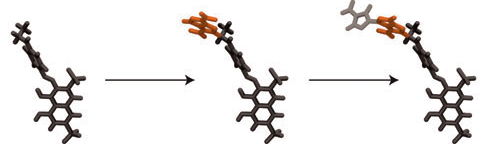
\includegraphics[width=\textwidth]{LigandSynthesis/Figures/Methods/Mutation.png}
  \label{subfig:SynthesisMutation}
}
\subfigure[Crossover by exchanging parts of parent ligands.]
{
  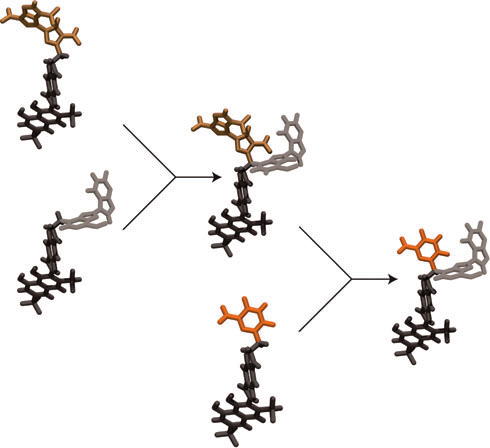
\includegraphics[width=\textwidth]{LigandSynthesis/Figures/Methods/Crossover.png}
  \label{subfig:SynthesisCrossover}
}
\caption{Illustration of the genetic operators of mutation and crossover used by AutoGrow. Figures reprinted from \citep{466-2009}.}
\label{fig:SynthesisMutationCrossover}
\end{figure}

\begin{figure}
\centering
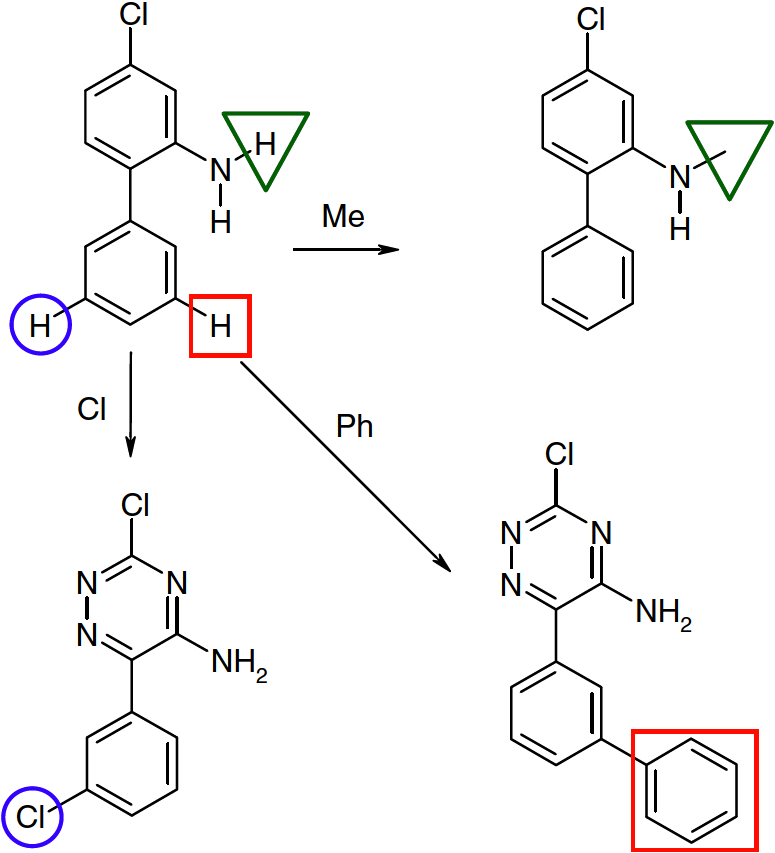
\includegraphics[width=\textwidth]{LigandSynthesis/Figures/Methods/HydrogenReplacement.png}
\caption{Examples of hydrogen replacement. Figure reprinted from \citep{325-2009}.}
\label{fig:HydrogenReplacement}
\end{figure}

\section{Method}

SmartGrow inherits from AutoGrow the existing crossover and mutation operators, and meanwhile implements two additional genetic operators, split and merging. The split operator breaks down a big ligand into two smaller but diverse pieces, while the merging operator combines two ligands into one. These two newly-invented operators remarkably increase the ligand diversity.

SmartGrow implements Lipinski's \textit{Rule of Five} \citep{169-1997,167-2000,168-2004} for drug likeness testing. Generated ligands that do not satisfy the rules are likely to be discarded. Its flexible program design allows future incorporation of new constraints.

SmartGrow incorporates a robust parser to correctly handle two-letter chemical elements such as Cl and Br, and adds additional support for phosphorus, further enhancing ligand diversity.

SmartGrow introduces a new concept called docking frequency to shorten the evaluation time. Evaluation by docking is performed every N generations, where N can be customized by the users, while for the other generations, evaluation is done by scoring only without true docking, a common major bottleneck of synthesis programs. When docking frequency is set to one, evaluation by docking occurs for all the generations, equivalent to the default behavior of AutoGrow. When docking frequency is larger than one, the initial ligand must first be docked against the protein to ensure evaluation by scoring is meaningful. Note that this preprocessing should be done before running SmartGrow.

Figure \ref{fig:SmartGrowFlowchart} shows the overall flowchart of SmartGrow. During initialization, the initial ligand serves as a core scaffold and is randomly mutated into multiple ligands by appending different fragments to different parts of the scaffold. Then Vina is invoked to evaluate the generated ligands either by docking or scoring, depending on the docking frequency. Ligands are sorted in the ascending order of predicted free energy, and control parameters are calculated for subsequent steps. Then mutation and split take place. Any one of the best ligands undergoes mutation and split, as shown on the right path. Afterwards, crossover and merging take place. Any two of the best ligands undergo crossover and merging, as shown on the left path. No matter which path, the generated ligands are examined by the guidance of Lipinski's \textit{Rule of Five}. Poor ligands are discarded should they violate two of the four rules. The passing ligands survive into the subsequent generation, and evaluation repeats until a given number of generations has reached.

\begin{figure}
\centering
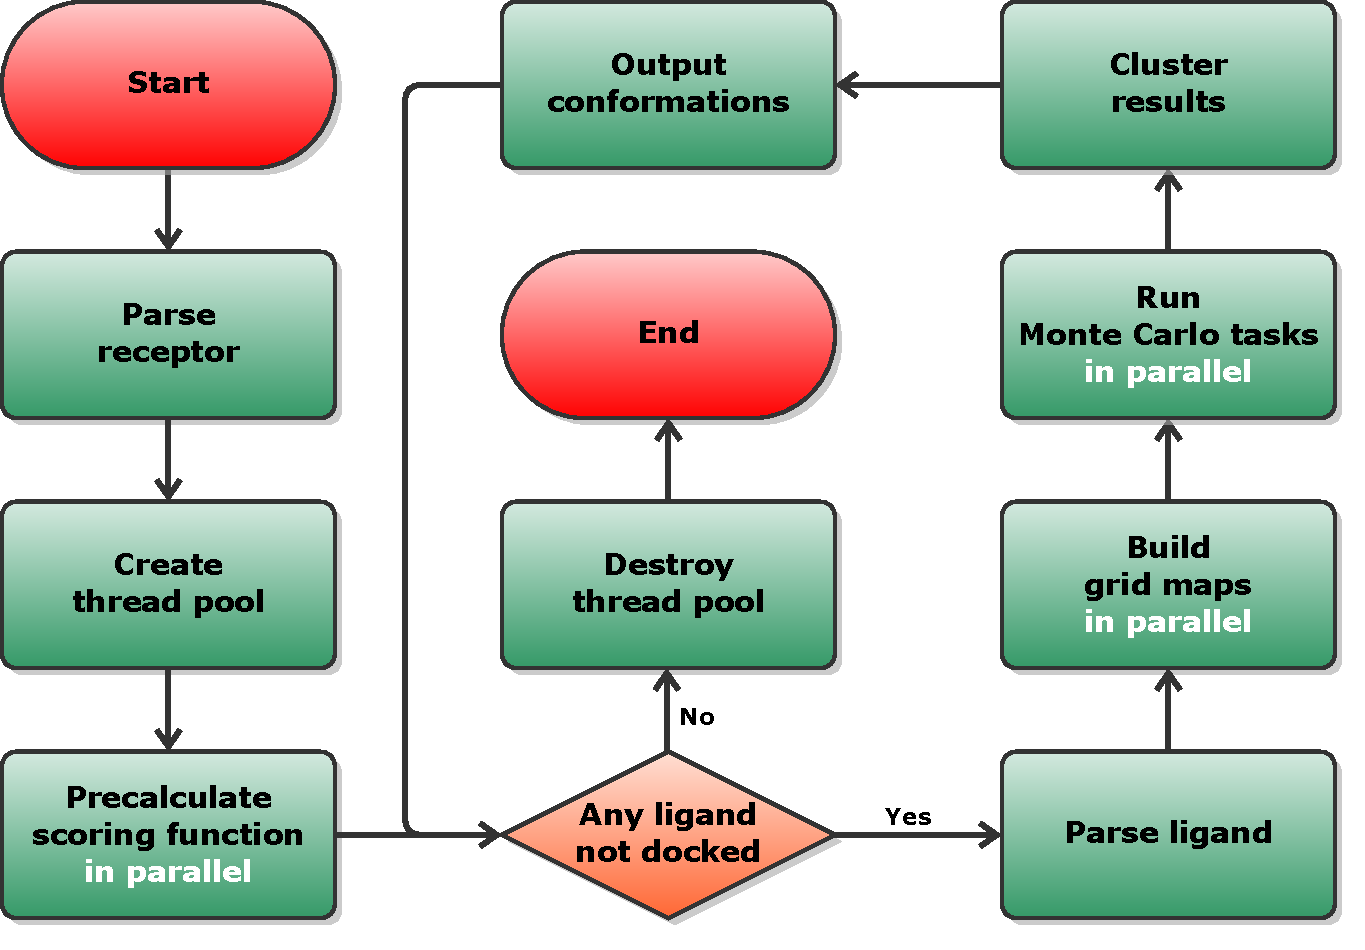
\includegraphics[width=\textwidth]{LigandSynthesis/Figures/Methods/Flowchart.pdf}
\caption{Flowchart of SmartGrow.}
\label{fig:SmartGrowFlowchart}
\end{figure}

Figure \ref{fig:GeneticOperators} illustrates the four genetic operators inside the genetic algorithm of SmartGrow. I stands for initial ligand, while A, B, and C stand for fragments. The common characteristic shared by all the four operators is that they retain the initial ligand as part of any generated ligand. In order words, the core scaffold of initial ligand must appear in all the generated ligands regardless of generation.

\begin{figure}
\centering
\subfigure[Mutation.]
{
  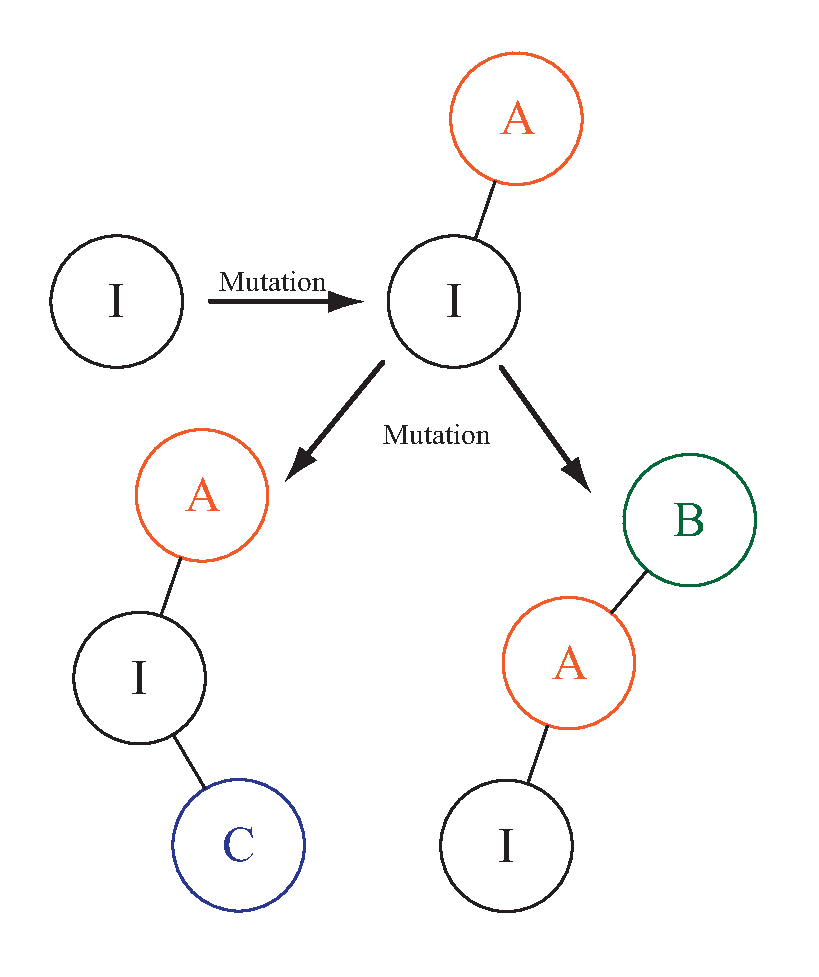
\includegraphics[width=0.41\textwidth]{LigandSynthesis/Figures/Methods/mutation.eps}
  \label{subfig:Mutation}
}
\subfigure[Crossover.]
{
  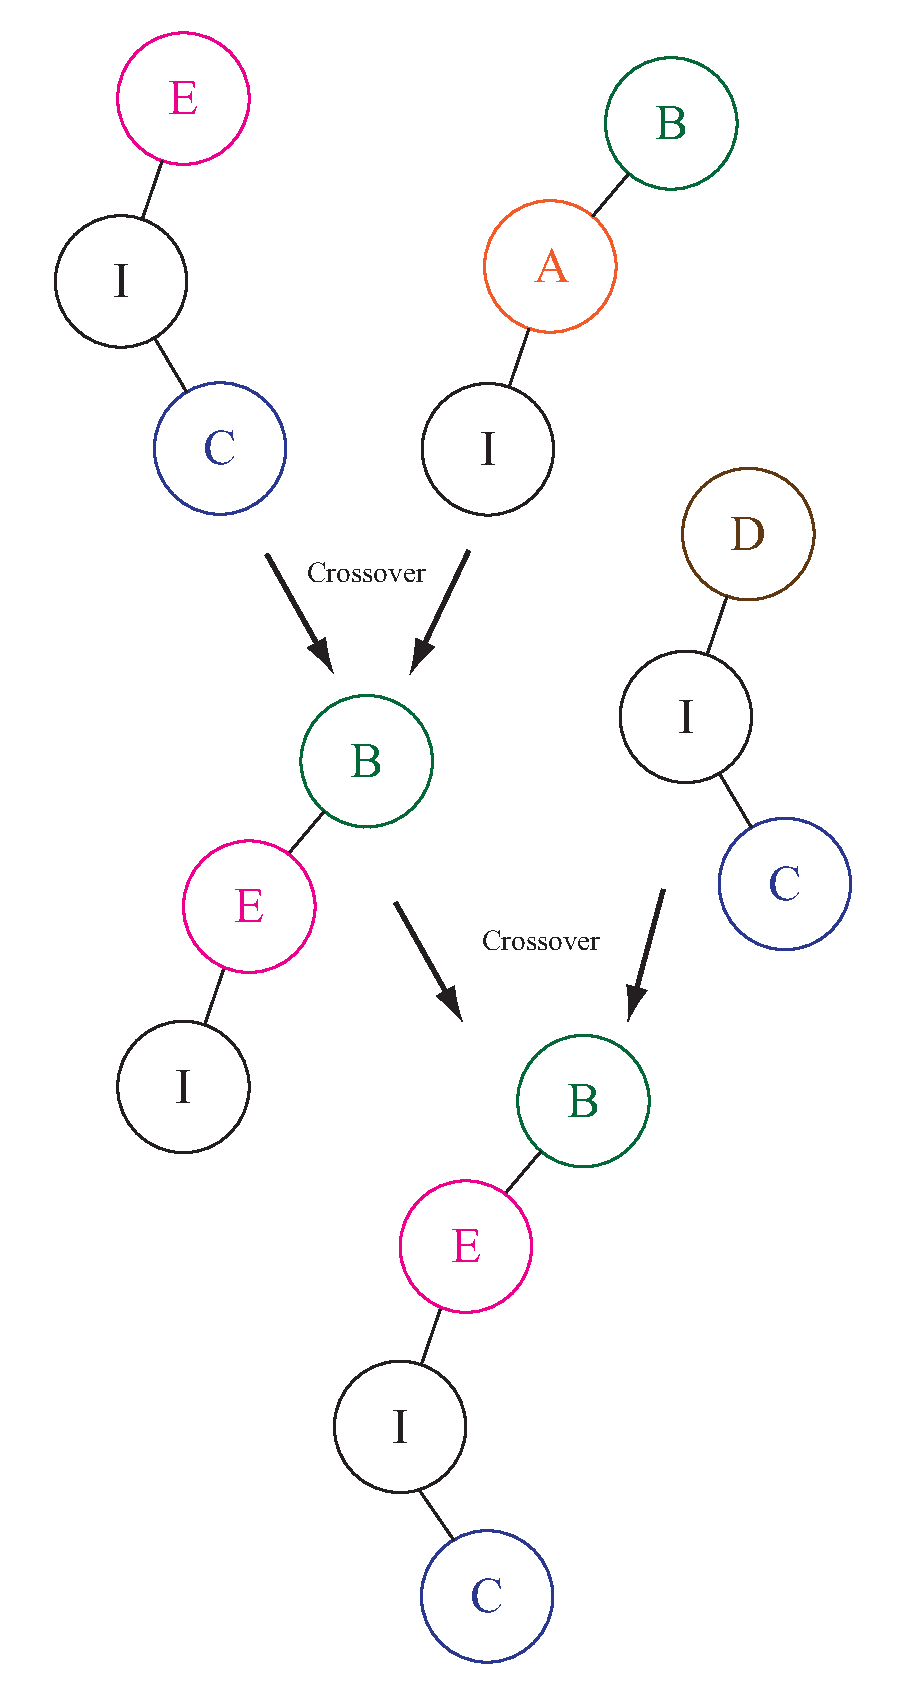
\includegraphics[width=0.41\textwidth]{LigandSynthesis/Figures/Methods/crossover.eps}
  \label{subfig:Crossover}
}
\subfigure[Split.]
{
  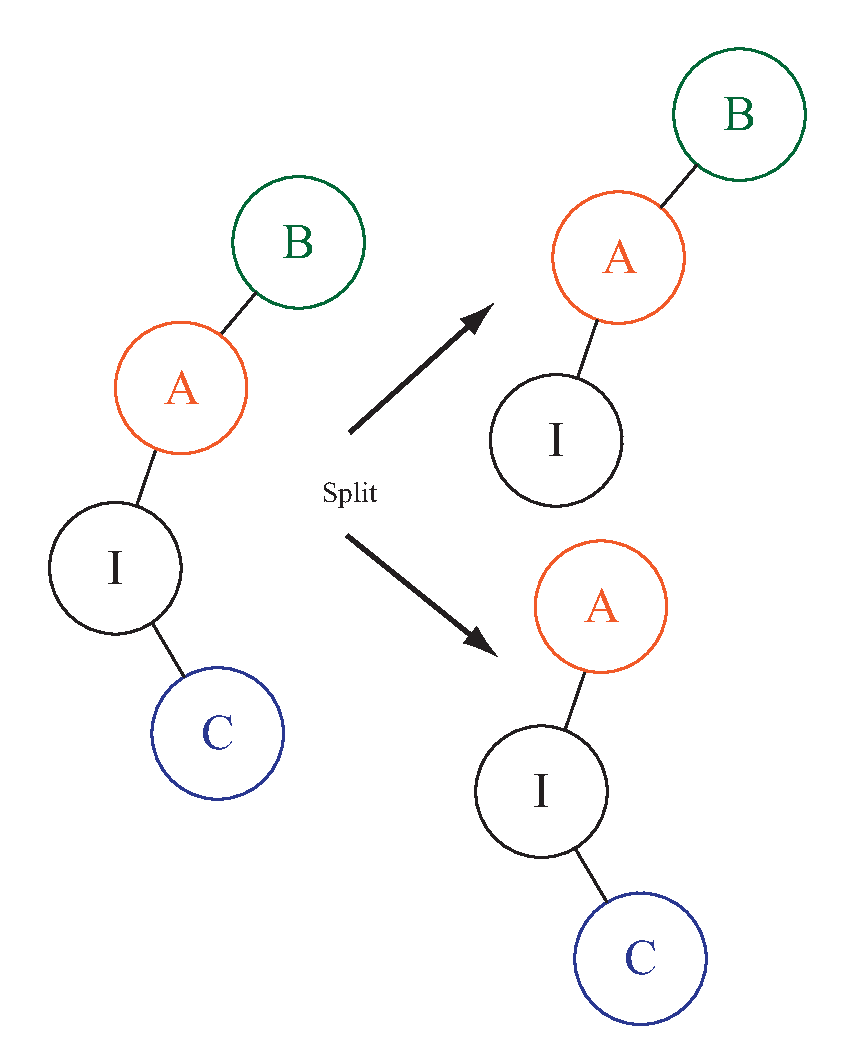
\includegraphics[width=0.41\textwidth]{LigandSynthesis/Figures/Methods/split.eps}
  \label{subfig:Split}
}
\subfigure[Merging.]
{
  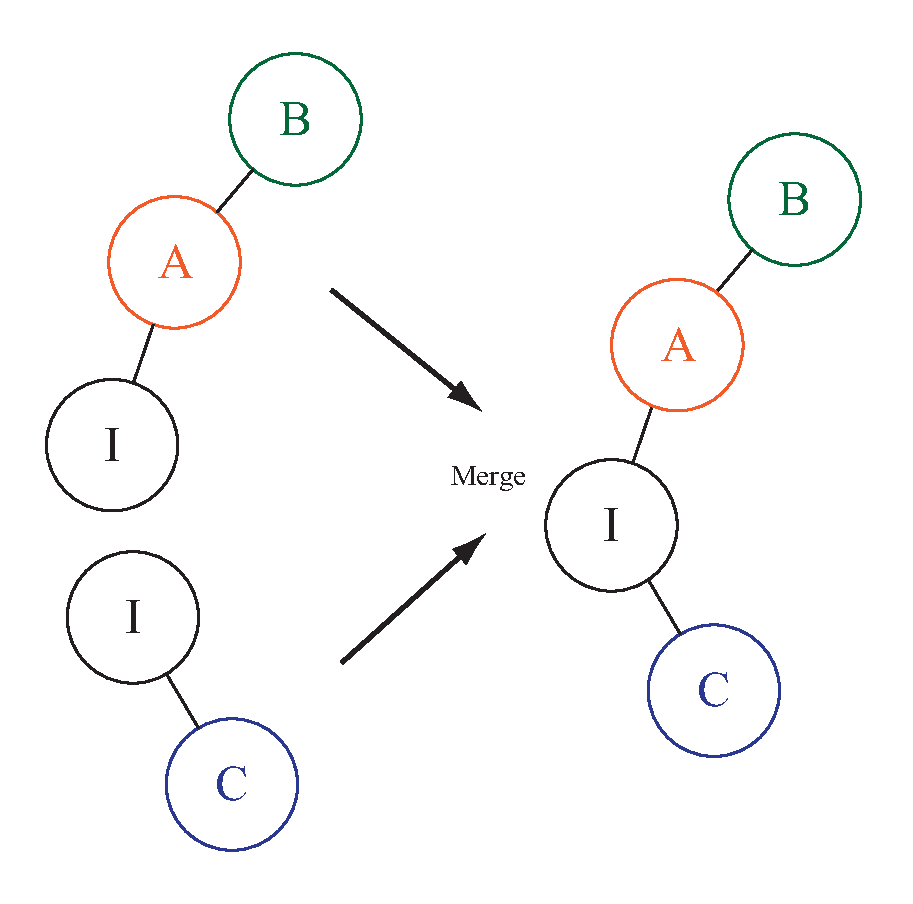
\includegraphics[width=0.41\textwidth]{LigandSynthesis/Figures/Methods/merging.eps}
  \label{subfig:Merging}
}
\caption{Illustrations of the genetic operators of mutation, crossover, split, and merging.}
\label{fig:GeneticOperators}
\end{figure}

\subsection{Selection}

The selection operator is based on Vina to calculate the fitness, which is in essence the predicted binding affinity. Individuals are ranked accordingly to their predicted free energy. The highest ranked ligands are directly carried over to the next generation.

\subsection{Mutation}

To mutate a ligand is to append a new fragment to it (Figures \ref{subfig:SynthesisMutation} and \ref{subfig:Mutation}). During mutation, a fragment is randomly retrieved from the fragment library. For both the ligand to mutate and the selected fragment, an appropriate hydrogen atom is randomly selected and denoted as linker hydrogen. A new mutant ligand is created by linking the ligand and fragment through their respective linker hydrogens, and replacing those two linker hydrogens by a single bond (Figure \ref{fig:HydrogenReplacement} \citep{325-2009}). Obviously mutation causes the molecular weight to increase.

This operator is used to create the initial population from the initial scaffold. It also rotates the bonds of the scaffold such that the resultant ligand is in its native conformation, where the pairwise distances among all atoms are maximized.

\subsection{Crossover}

During crossover, two parent ligands are first randomly chosen from a collection of best ligands. Since every ligand in the population retains the same scaffold of initial ligand, this scaffold acts as a crossover point and will be retained in the generated offspring. The remaining fragments of the parents are randomly chosen to append to the offspring (Figure \ref{subfig:Crossover}). As each parent ligand may contain a different set of fragments, the produced offspring can be significantly different by mixing the sets of fragments, but meanwhile maintain the quality of its parents. Crossover may increase or decrease the molecular weight.

\subsection{Split}

To split a ligand is to simply break it down into two smaller pieces. During split, the core scaffold of the ligand must first be identified, hence another ligand, which also retains the core scaffold, is randomly chosen as reference. The overlapping part of both ligands forms the scaffolds of the two children ligands. The remaining fragments of the ligand to split are then randomly distributed to the two children (Figure \ref{subfig:Split}). Obviously split causes the molecular weight to decrease.

The split operator is in fact a very essential operator that distinguishes SmartGrow apart from AutoGrow. It was introduced with the purpose to address the problem of generating excessively large ligands by mutation. As mutations always append new fragments, the ligands grow larger and larger. The invention of the split operator tackles this kind of early convergence problem.

\subsection{Merging}

To merge two ligands, the identical core scaffold of both ligands remains, and the remaining fragments of both ligands are appended to the generated ligand (Figure \ref{subfig:Merging}). Obviously merging causes the molecular weight to increase, even more significantly than mutation.

\subsection{Drug Likeness Testing}

SmartGrow implements Lipinski's \textit{Rule of Five} as a guideline to ensure the generated ligands carry drug-like properties. As summarized by Lipinski, a ligand is drug like if and only if the following conditions hold: 1) its molecular weight is within 0 to 500 Da, 2) its number of hydrogen bond donors is within 0 to 5, 3) its number of hydrogen bond acceptors is within 0 to 10, and 4) its octanol-water partition coefficient, denoted as LogP, is within 0 to 5. The first three rules are easy to implement. For the calculation of LogP, SmartGrow implements MLogP, which uses the sum of lipophilic and hydrophilic atoms as two basic descriptors, plus 11 correction factors. MLogP was chosen rather than other algorithms because it is rule-based and fits perfectly into the data structure of SmartGrow. To maintain diversity, a ligand is only rejected if it cannot satisfy any two rules.

\section{Data}

In order to fully test SmartGrow, 18 comprehensive testcases were collected, including 3 proteins, 8 initial ligands, and a library containing 46 small fragments.

\subsection{Proteins}

We aimed to select proteins that are of real-life importance. Glycogen synthase kinase 3 beta (GSK3$\beta$) is a theoretically promising pharmacotherapeutic target for the treatment of several human diseases, including cancer, type-2 diabetes \citep{247-2004} and Alzheimer's disease (AD) \citep{248-2006}. Efforts into discovering new inhibitors of GSK3$\beta$ never stop \citep{704-2010,728-2011,729-2011,760-2011}. Therefore it was included into our test data.
% A New Protocol for Predicting Novel GSK-3b ATP Competitive Inhibitors

HIV also caught our eye sights because of its worldwide impact. Researchers have spent over 30 years in studying HIV \citep{300-2010,322-2010,318-2010,683-2011}. HIV reverse transcriptase (HIV RT) \citep{315-2009,312-2010,323-2010,730-2011,314-2011,320-2011,505-2011} and HIV protease (HIV PR) \citep{309-2010,673-2011,671-2011,731-2011,504-2010,556-2010}, two viral enzymes residing in the body of the virus assisting in infecting human cells, were also included into our test data.

In total, three proteins were collected from the Protein Data Bank (PDB) database \citep{540-2000,539-2000,537-2003,105-2007,538-2008} for testing. The three proteins were manually extracted out of their complexes. Catalytic Site Altas (CSA) \citep{209-2004} and relevant publications \citep{245-2004,247-2004,248-2006,704-2010,300-2010,322-2010,318-2010,321-2008,504-2010} were queried for their possible binding sites (Table \ref{tab:SynthesisSearchSpace}), which are defined as cuboid box determined by center coordinate together with width, height, and depth.

\begin{table}
\centering
\begin{tabular*}
{\textwidth}
{@{\extracolsep{\fill}}ccccc}
\toprule
PDB ID & Protein & Resolution (\AA) & Box center (\AA) & Box size (\AA)\\
\midrule
1J1B & GSK3$\beta$ & 1.80 & (20.304, 16.365, -9.814)  & (22, 18 ,20)\\
2ZD1 & HIV RT      & 1.80 & (49.712, -28.441, 35.555) & (16, 16, 18)\\
3KFN & HIV PR      & 1.77 & (8.113, 9.701, 4.310)     & (22, 26, 22)\\
\bottomrule
\end{tabular*}
\caption{PDB IDs, resolutions, box centers and sizes of GSK3$\beta$, HIV RT, and HIV PR.}
\label{tab:SynthesisSearchSpace}
\end{table}

\subsection{Initial Ligands}

We aimed to select initial ligands that spread across a wide range of free energies and molecular weights. The three ligands of PDB heterogeneous molecule IDs TRS, T27 \citep{299-2005,321-2008}, and 4DX are respectively the native ligands of GSK3$\beta$, HIV RT, and HIV PR, hence they were included. Additionally, five more ligands were retrieved from the ZINC database \citep{532-2005}. The free energies and molecular weights of these five ligands are in different ranges. They cover a relatively complete value domain, and were thus included. Figure \ref{fig:InitialLigands} summarizes the eight selected initial ligands. MW stands for molecular weight.

\begin{figure}
\centering
\subfigure[TRS (MW = 122 Da)]
{
  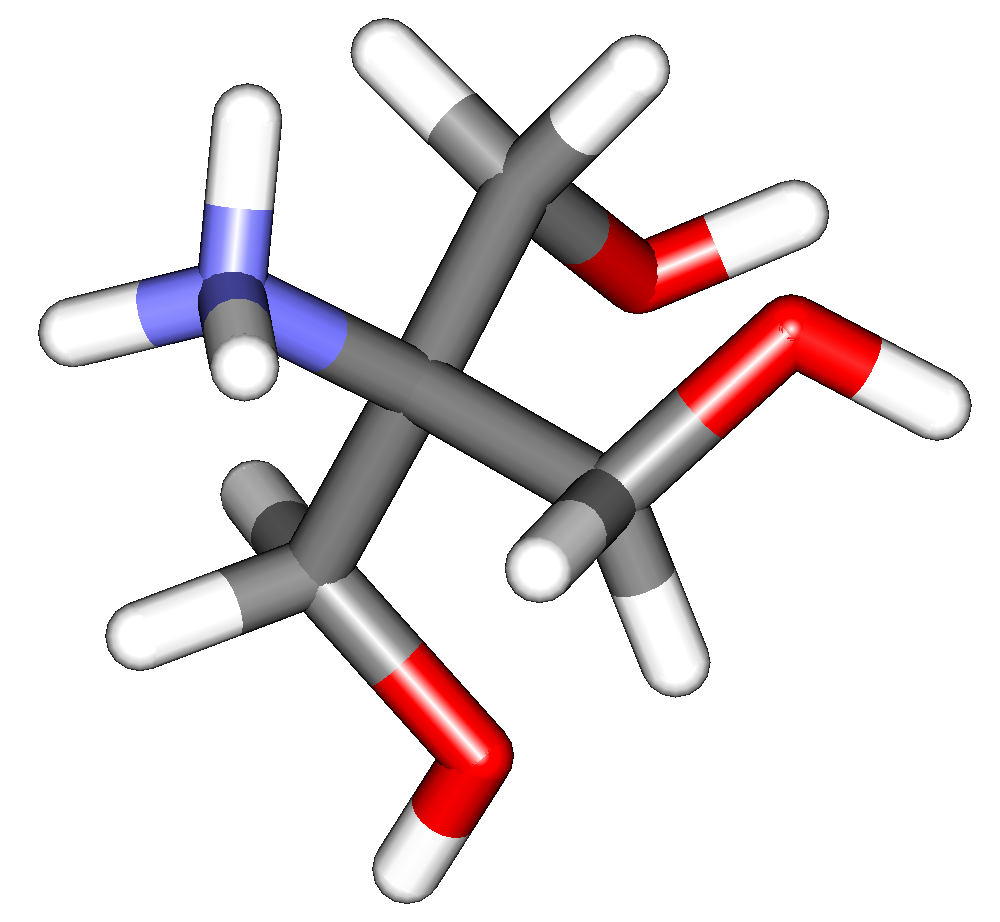
\includegraphics[width=0.3\textwidth]{LigandSynthesis/Figures/Ligands/TRS.png}
  \label{subfig:Ligands-TRS}
}
\subfigure[T27 (MW = 373 Da)]
{
  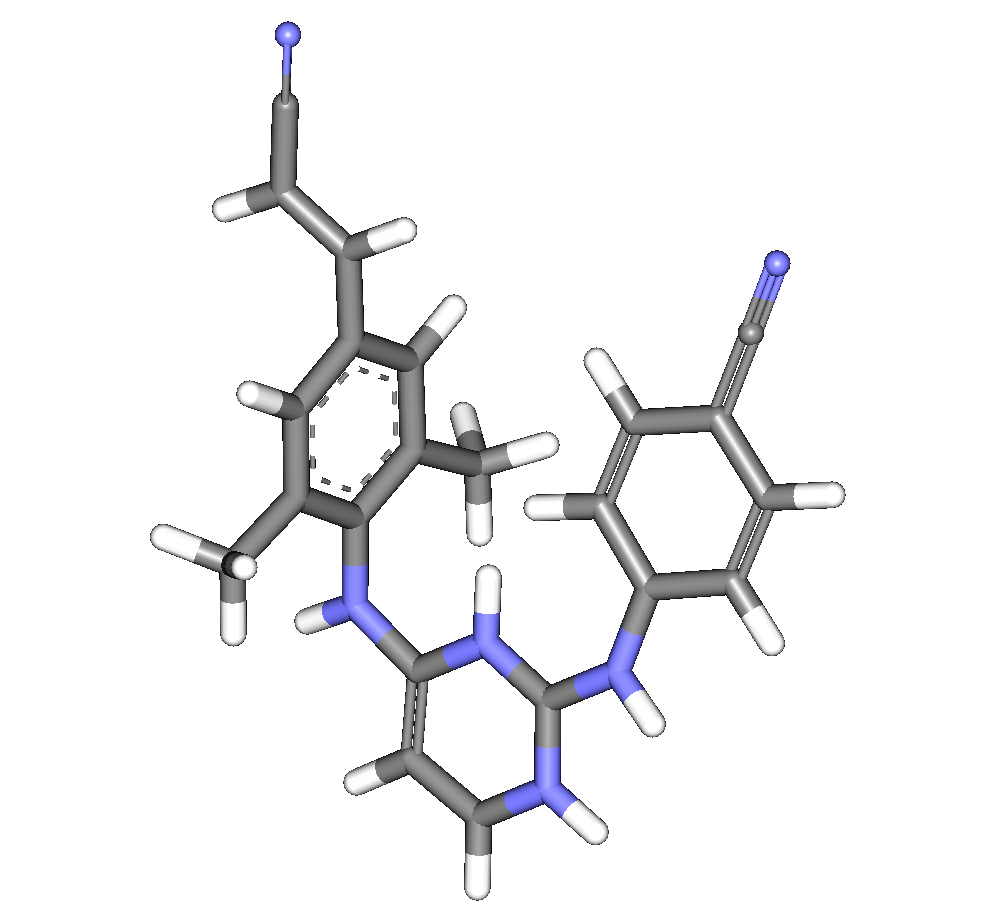
\includegraphics[width=0.3\textwidth]{LigandSynthesis/Figures/Ligands/T27.png}
  \label{subfig:Ligands-T27}
}
\subfigure[4DX (MW = 114 Da)]
{
  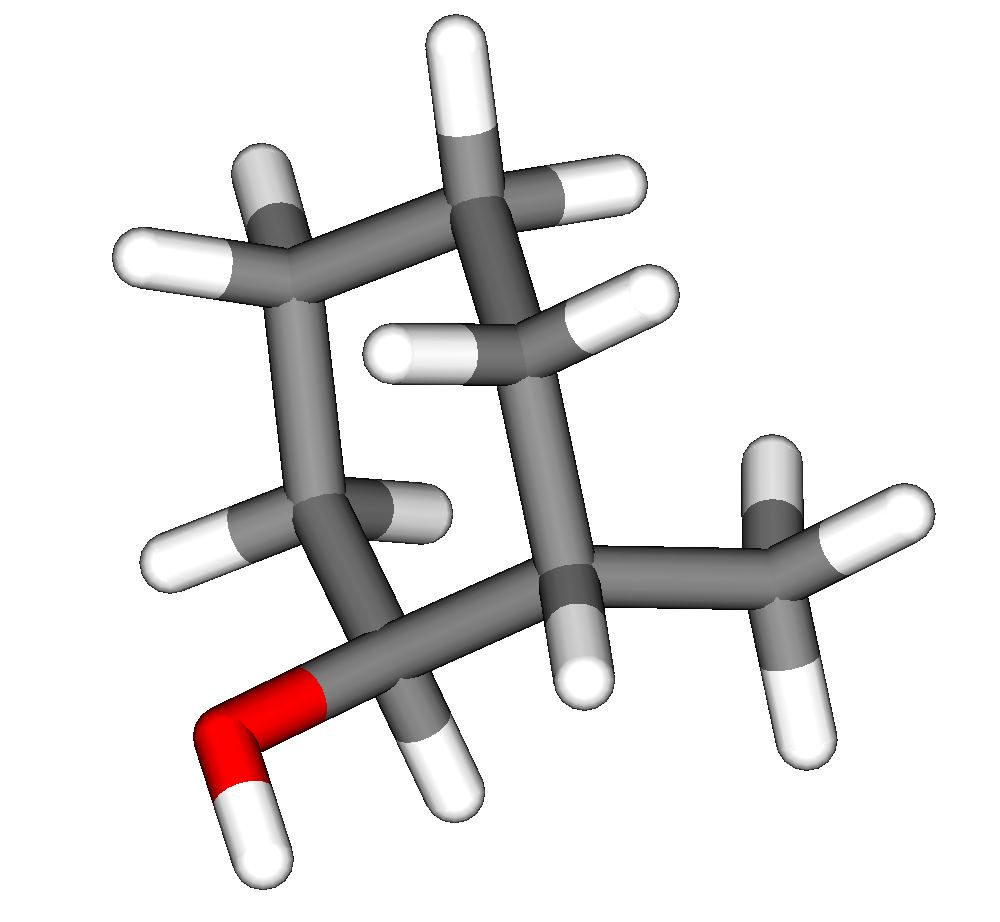
\includegraphics[width=0.3\textwidth]{LigandSynthesis/Figures/Ligands/4DX.png}
  \label{subfig:Ligands-4DX}
}
\subfigure[ZINC01019824 (MW = 194 Da)]
{
  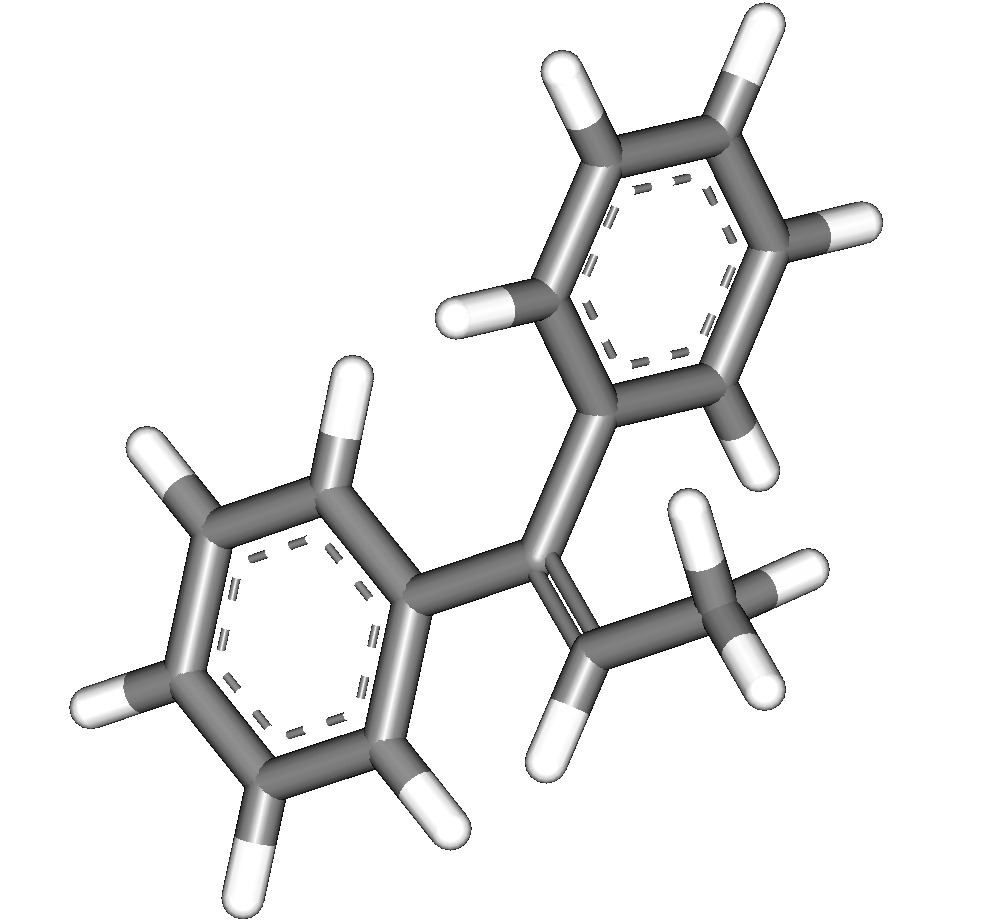
\includegraphics[width=0.3\textwidth]{LigandSynthesis/Figures/Ligands/ZINC01019824.png}
  \label{subfig:Ligands-ZINC01019824}
}
\subfigure[ZINC08442219 (MW = 224 Da)]
{
  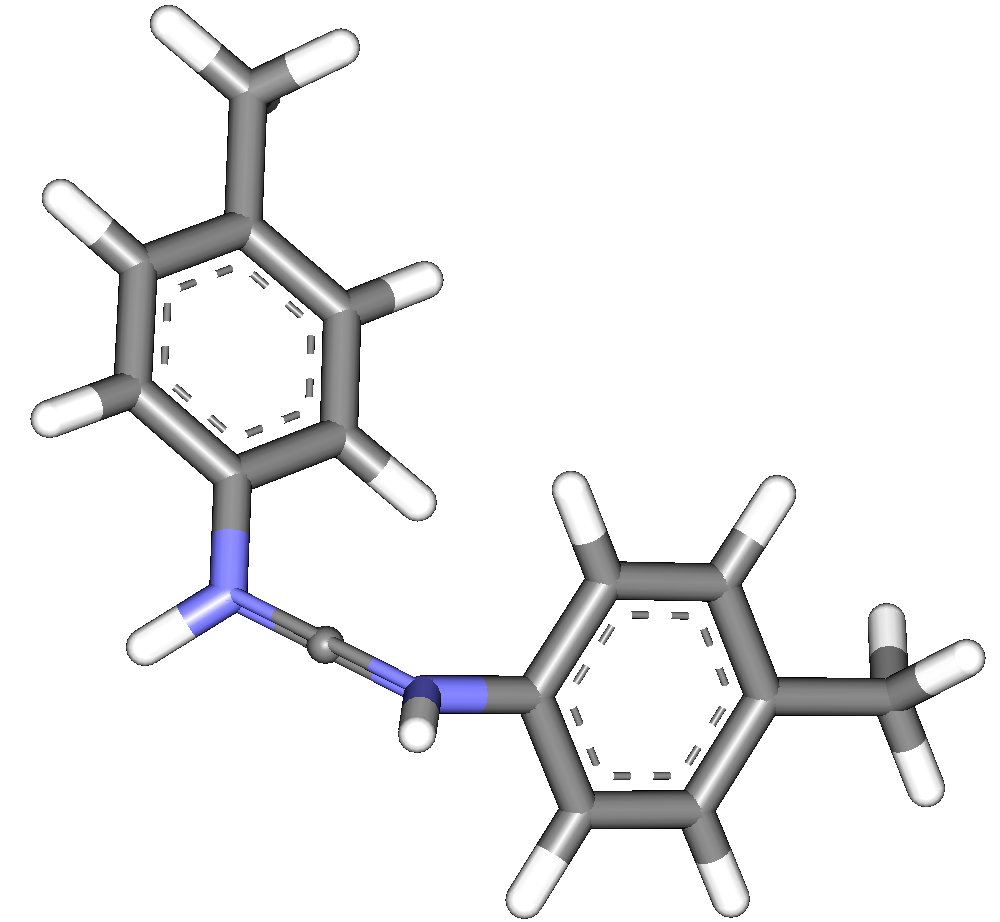
\includegraphics[width=0.3\textwidth]{LigandSynthesis/Figures/Ligands/ZINC08442219.png}
  \label{subfig:Ligands-ZINC08442219}
}
\subfigure[ZINC09365179 (MW = 278 Da)]
{
  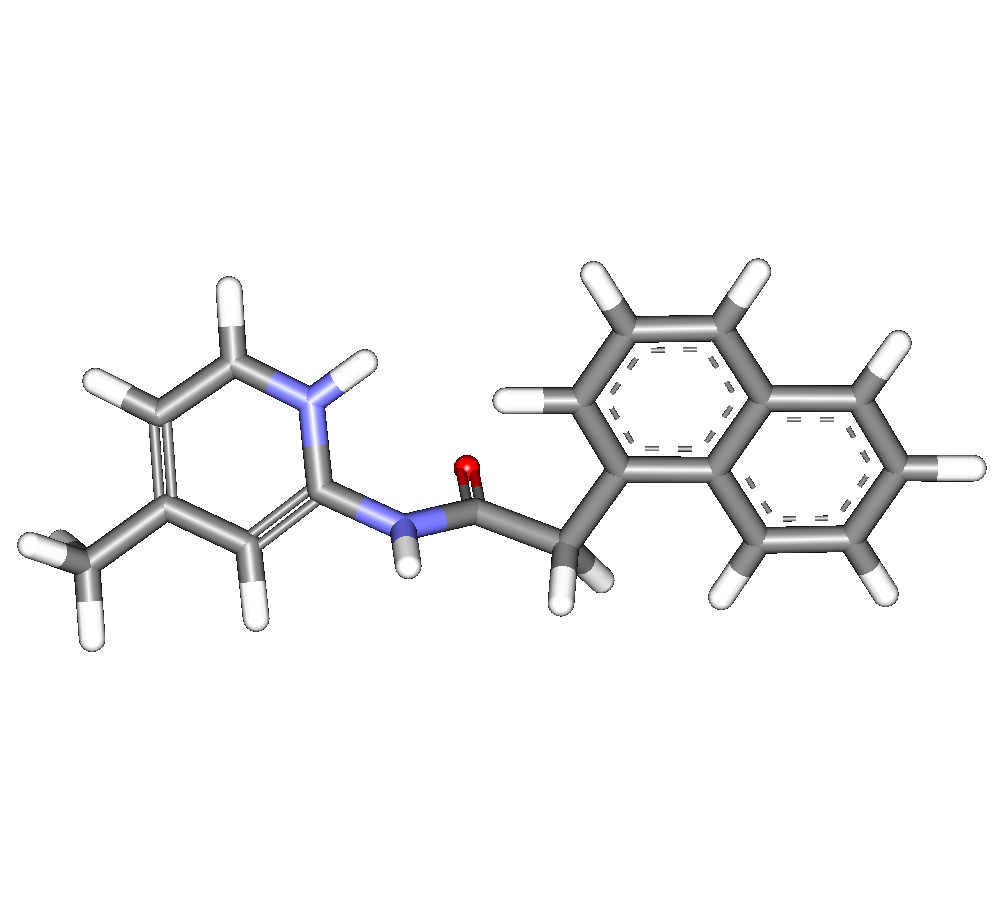
\includegraphics[width=0.3\textwidth]{LigandSynthesis/Figures/Ligands/ZINC09365179.png}
  \label{subfig:Ligands-ZINC09365179}
}
\subfigure[ZINC18153302 (MW = 142 Da)]
{
  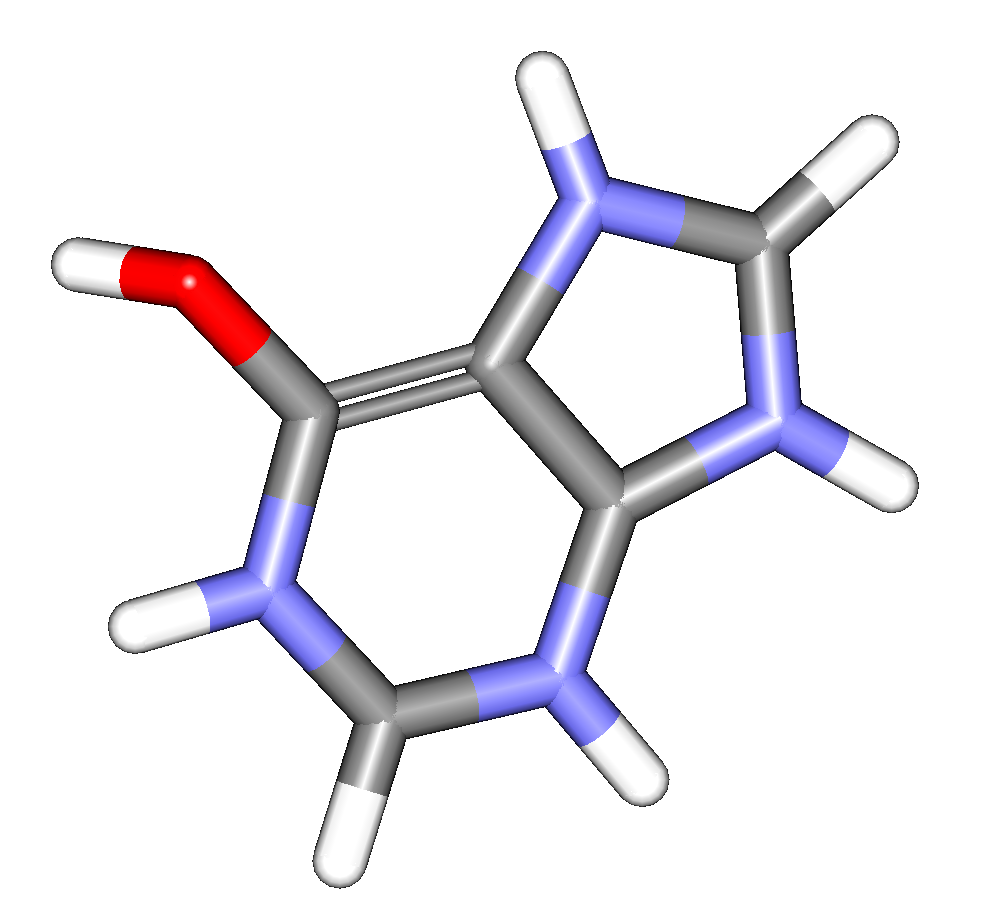
\includegraphics[width=0.3\textwidth]{LigandSynthesis/Figures/Ligands/ZINC18153302.png}
  \label{subfig:Ligands-ZINC18153302}
}
\subfigure[ZINC20030231 (MW = 209 Da)]
{
  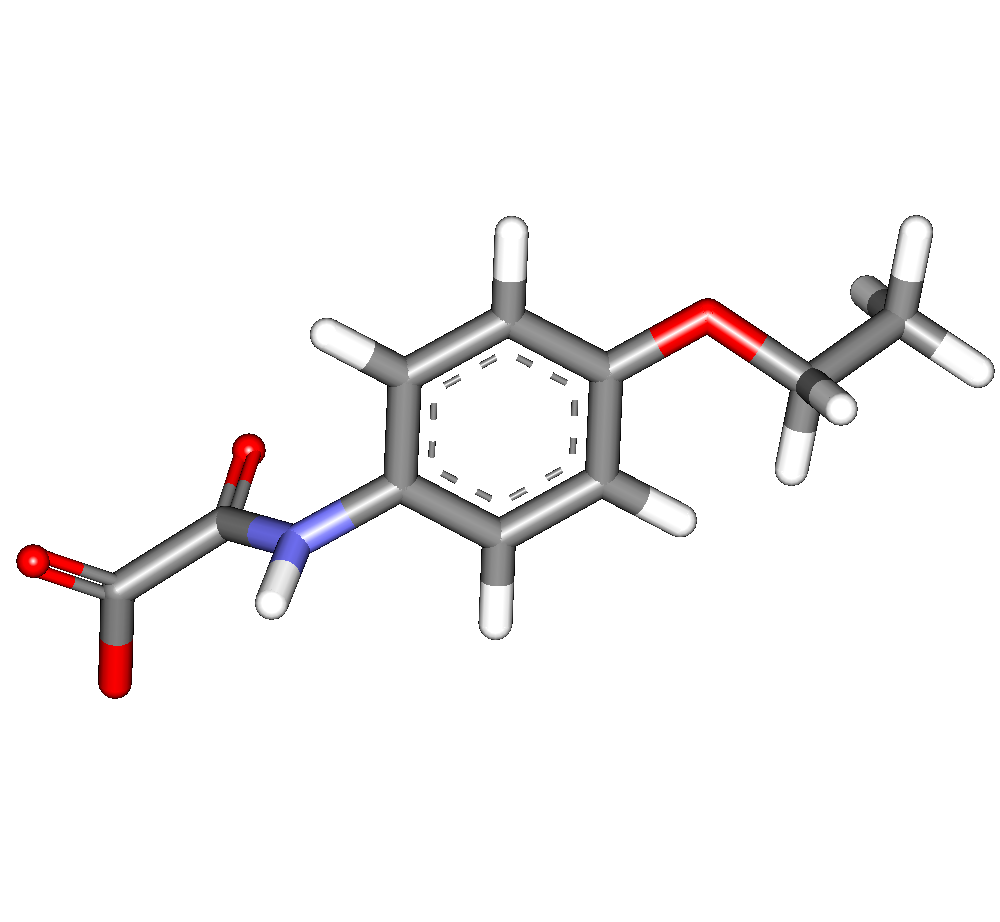
\includegraphics[width=0.3\textwidth]{LigandSynthesis/Figures/Ligands/ZINC20030231.png}
  \label{subfig:Ligands-ZINC20030231}
}
\caption{Stick representations and molecular weights of the eight unique initial ligands.}
\label{fig:InitialLigands}
\end{figure}

\subsection{Fragments}

Ligands are mutated by appending new fragments from a fragment library, which can be constructed by various means \citep{470-2009,751-2011,656-2011}. There are two fragment libraries that accompanied with the release of AutoGrow, namely the small-fragment library and the large-fragment library. We tested both libraries internally, and noticed early convergence when using the large-fragment library, which turned out to be quite problematic for testing purposes. So we focused on the small-fragment library, which is made up of 46 fragments. These fragments are generally small in size, having 3 to 15 atoms and an average of 9.6 atoms with a standard deviation of 2.8 (Figure \ref{fig:SmallFragmentLibrary} \citep{466-2009}).

\begin{figure}
\centering
\subfigure[The 46 small fragments.]
{
  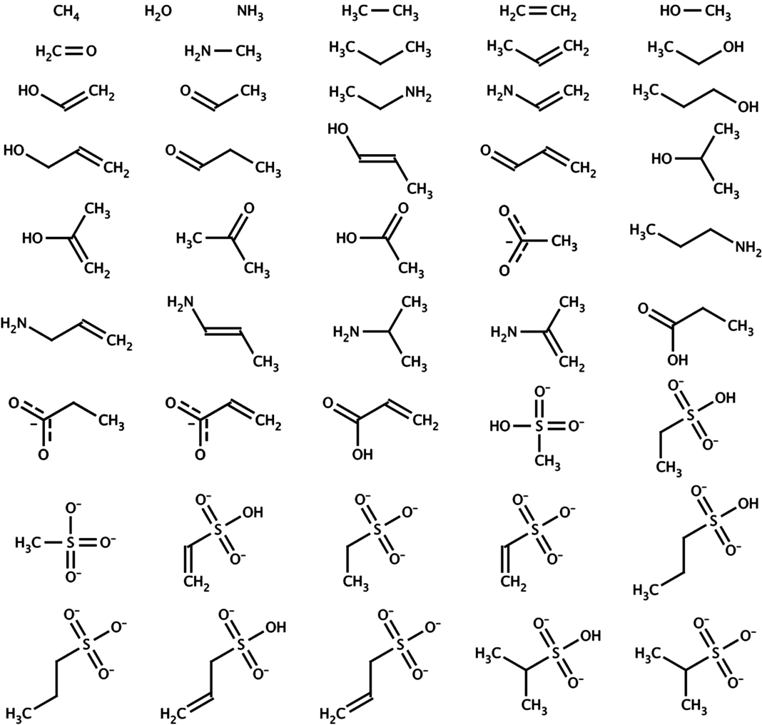
\includegraphics[width=0.75\textwidth]{LigandSynthesis/Figures/Methods/SmallFragments.png}
  \label{subfig:SmallFragments}
}
\subfigure[Distribution of number of atoms.]
{
  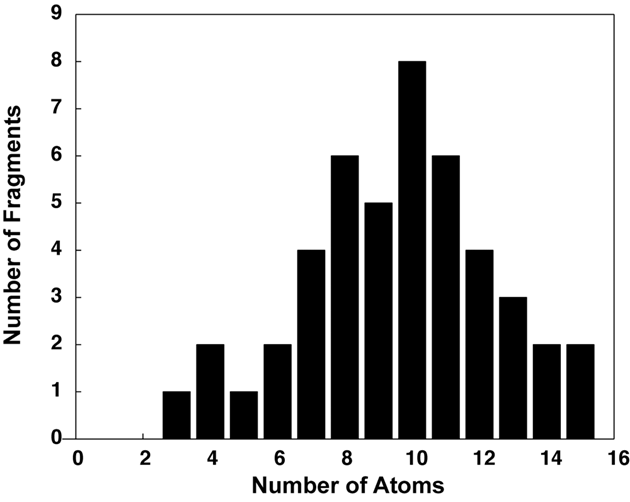
\includegraphics[width=0.75\textwidth]{LigandSynthesis/Figures/Methods/SmallFragmentLibraryStatistics.png}
  \label{subfig:SmallFragmentLibraryStatistics}
}
\caption{The small fragment library and distribution of number of atoms. Figures reprinted from \citep{466-2009}.}
\label{fig:SmallFragmentLibrary}
\end{figure}

\section{Experiments and Results}

The experiments include 1) validation of both programs to ensure generated ligands are chemically valid, 2) comparison of their synthesis performance in terms of predicted free energy, molecular weight, and execution time, and 3) evaluation of the support for phosphorus by SmartGrow.

We tested SmartGrow version 1.14 and compared it with AutoGrow version 2.0.4, the most recent versions of both programs at the moment this thesis was composed. To run both programs, we manually set up the running environment, including the installations of Java, Python, AutoDock Vina \citep{595-2010}, AutoDock Tools \citep{785-1999,596-2009}, and configurations of relevant scripts, initial ligands, search spaces, and fragment libraries. All these tasks are extremely messy, so it did cost us some time for correct configurations before successfully running the code.

Table \ref{tab:ParameterSettings} lists the parameter settings for AutoGrow and SmartGrow. Elitists refer to the best ligands of a generation that will survive directly into the next generation. Children refer to ligands generated by crossover. Mutants refer to ligands generated by mutation. The default values for AutoGrow were retained, i.e. 10, 20, 20, and 8 for the number of elitists, children, mutants, and generations, respectively. The docking frequency of AutoGrow is fixed to 1. The maximum number of atoms was set to 80 because we noticed from initial trials that the generated ligands of final generation consisted of around 70 atoms but their molecular weight already exceeded 500 Da, a threshold set by Lipinski's \textit{Rule of Five}. To make a fair comparison, the settings for SmartGrow were set to be identical as AutoGrow except for the number of generations and docking frequency. Since SmartGrow supports evaluation by scoring only, its docking frequency was set to 3 to examine this special feature. Meanwhile, the number of generations in which evaluation is done by true docking should be maintained to 8, which is the same as AutoGrow, the number of generations for SmartGrow was set to 24, the product of 3 and 8.

\begin{table}
\centering
\begin{tabular*}
{\textwidth}
{@{\extracolsep{\fill}}lrr}
\toprule
Program & AutoGrow & SmartGrow\\
\midrule
Number of elitists & 10 & 10\\
Number of children & 20 & 20\\
Number of mutants & 20 & 20\\
Number of generations & 8 & 24\\
Docking frequency & 1 & 3\\
Max number of atoms & 80 & 80\\
\bottomrule
\end{tabular*}
\caption{Parameter settings for AutoGrow and SmartGrow.}
\label{tab:ParameterSettings}
\end{table}

In summary, three proteins were collected, each of which is associated with 6 initial ligands. Therefore there are 18 testcases in total. Since genetic algorithm is stochastic, for each testcase we ran AutoGrow and SmartGrow for 9 times on six Linux machines with Intel Xeon Dual Quad Core 2.4GHz and 32GB RAM under Ubuntu 10.04.1 x86\_64. Each execution required approximately 2 hours on average, hence the whole test procedure cost about 2,592 CPU hours. One may run the testcases for 20 times for a more accurate comparison if time permitted.

\subsection{Binding Conformation}

To validate the correctness of ligands generated by both program, from each testcase we visualized the best ligand in complex of its associated protein. Figure \ref{fig:BestLigands} shows three testcases. Hydrogen bonds are represented by dotted green lines. Table \ref{tab:BestLigands} lists the predicted binding affinities.

\begin{figure}
\centering
\subfigure[GSK3$\beta$ in complex with ZINC01019824.]
{
  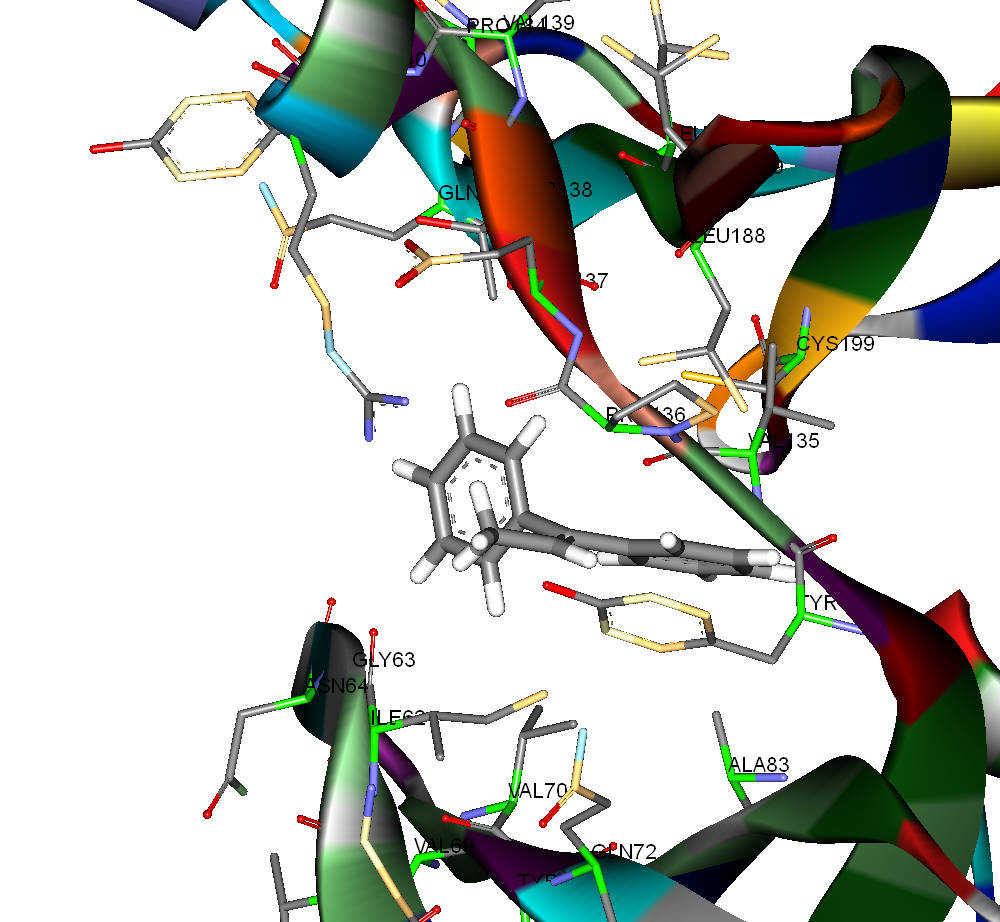
\includegraphics[width=0.3\textwidth]{LigandSynthesis/Figures/Results/1J1B-ZINC01019824.png}
  \label{subfig:1J1B-ZINC01019824}
}
\subfigure[GSK3$\beta$ in complex with the best ligand generated from ZINC01019824 by AutoGrow.]
{
  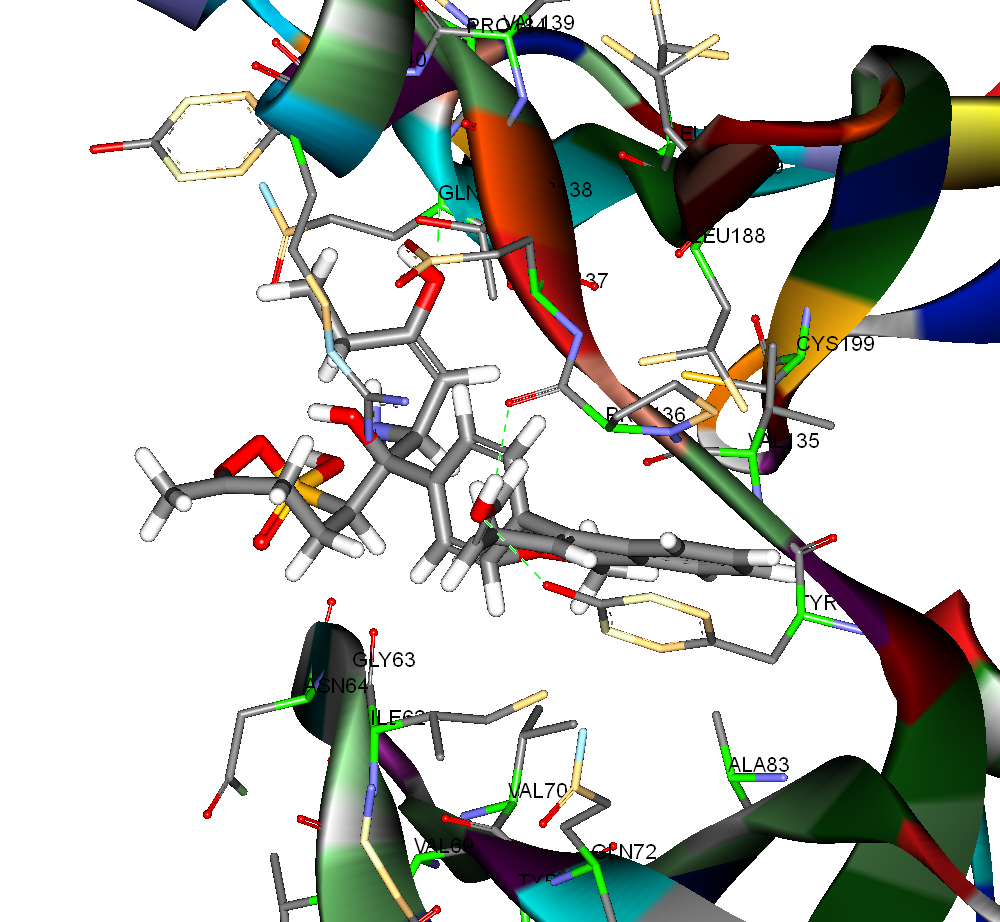
\includegraphics[width=0.3\textwidth]{LigandSynthesis/Figures/Results/1J1B-ZINC01019824-AutoGrow.png}
  \label{subfig:1J1B-ZINC01019824-AutoGrow}
}
\subfigure[GSK3$\beta$ in complex with the best ligand generated from ZINC01019824 by SmartGrow.]
{
  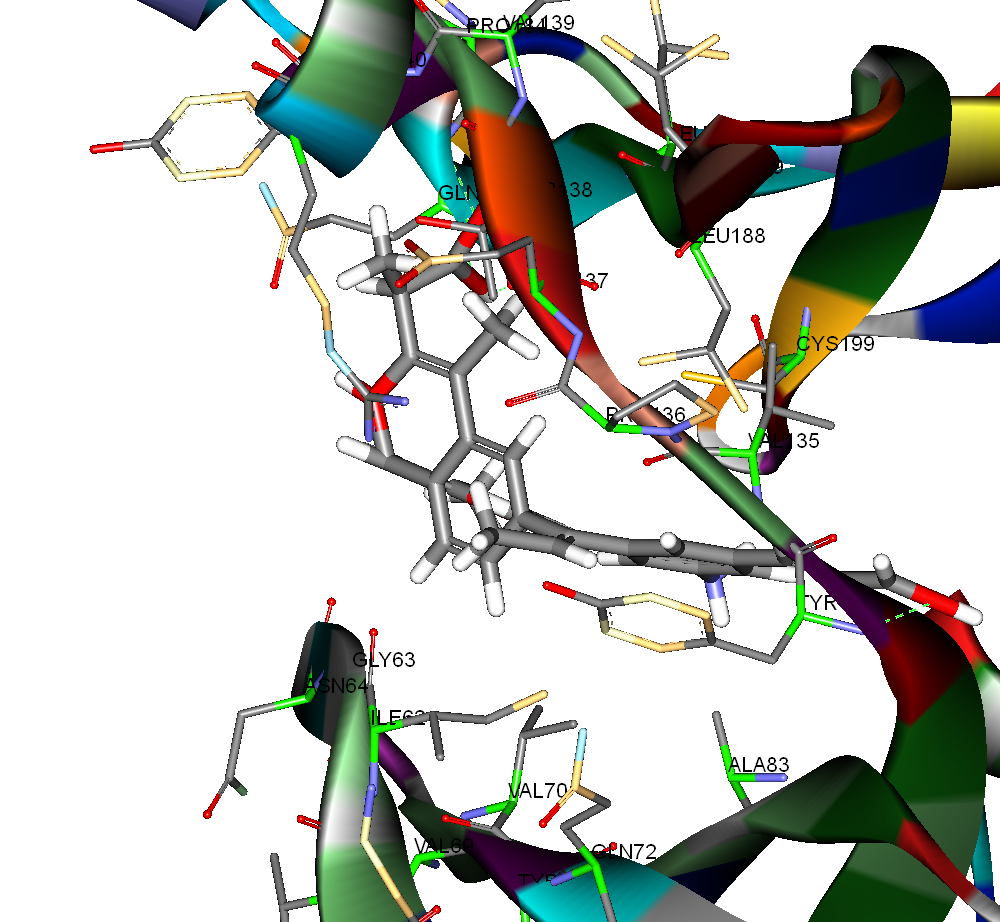
\includegraphics[width=0.3\textwidth]{LigandSynthesis/Figures/Results/1J1B-ZINC01019824-SmartGrow.png}
  \label{subfig:1J1B-ZINC01019824-SmartGrow}
}
\subfigure[HIV RT in complex with ZINC08442219.]
{
  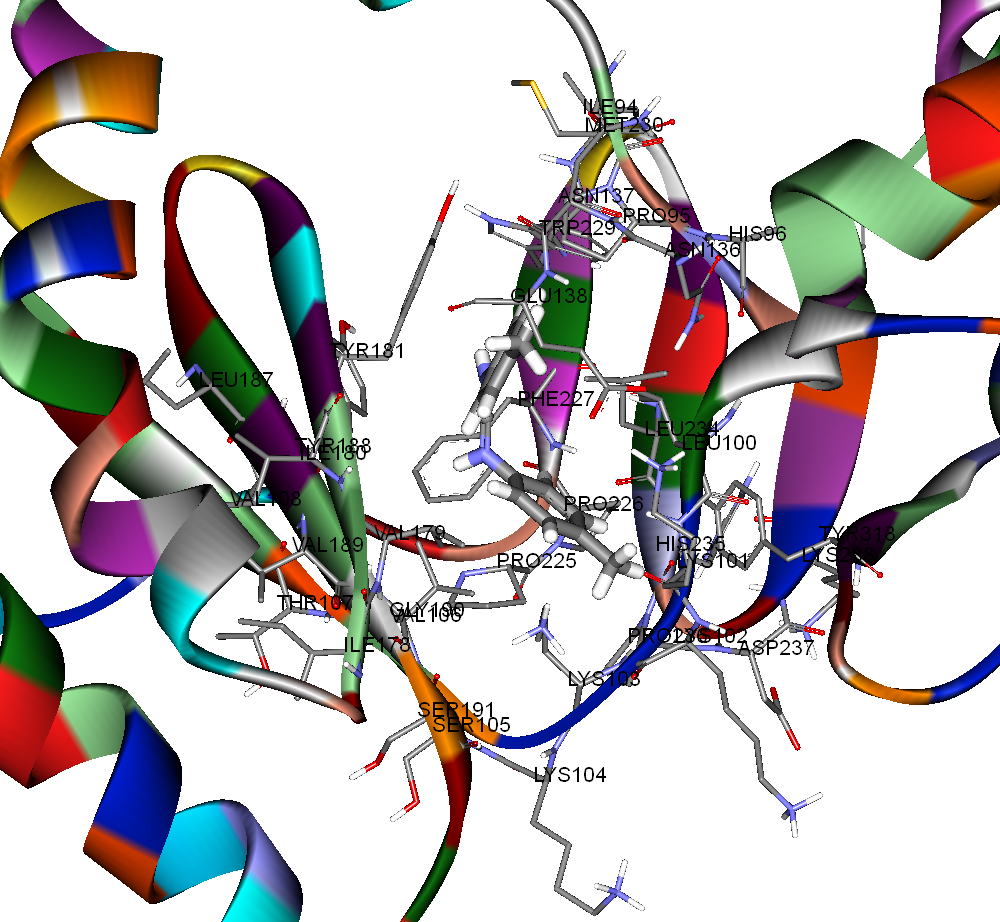
\includegraphics[width=0.3\textwidth]{LigandSynthesis/Figures/Results/2ZD1-ZINC08442219.png}
  \label{subfig:2ZD1-ZINC08442219}
}
\subfigure[HIV RT in complex with the best generated ligand from ZINC08442219 by AutoGrow.]
{
  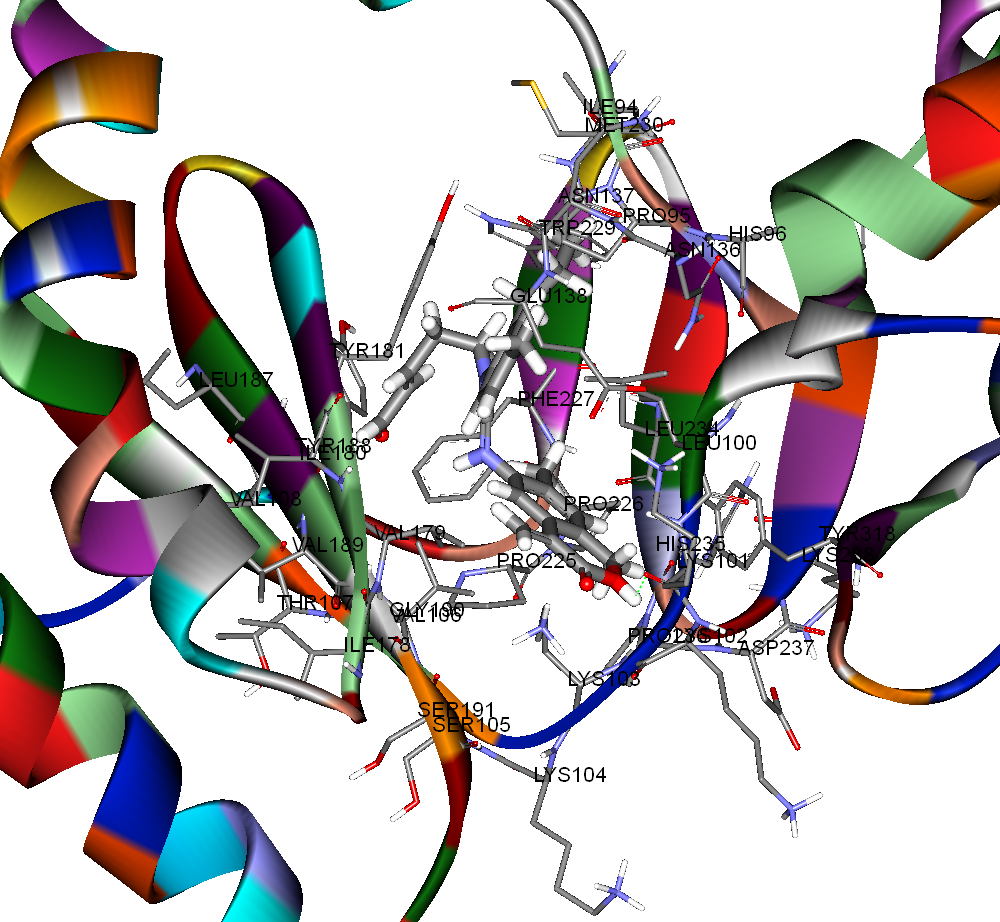
\includegraphics[width=0.3\textwidth]{LigandSynthesis/Figures/Results/2ZD1-ZINC08442219-AutoGrow.png}
  \label{subfig:2ZD1-ZINC08442219-AutoGrow}
}
\subfigure[HIV RT in complex with the best generated ligand from ZINC08442219 by SmartGrow.]
{
  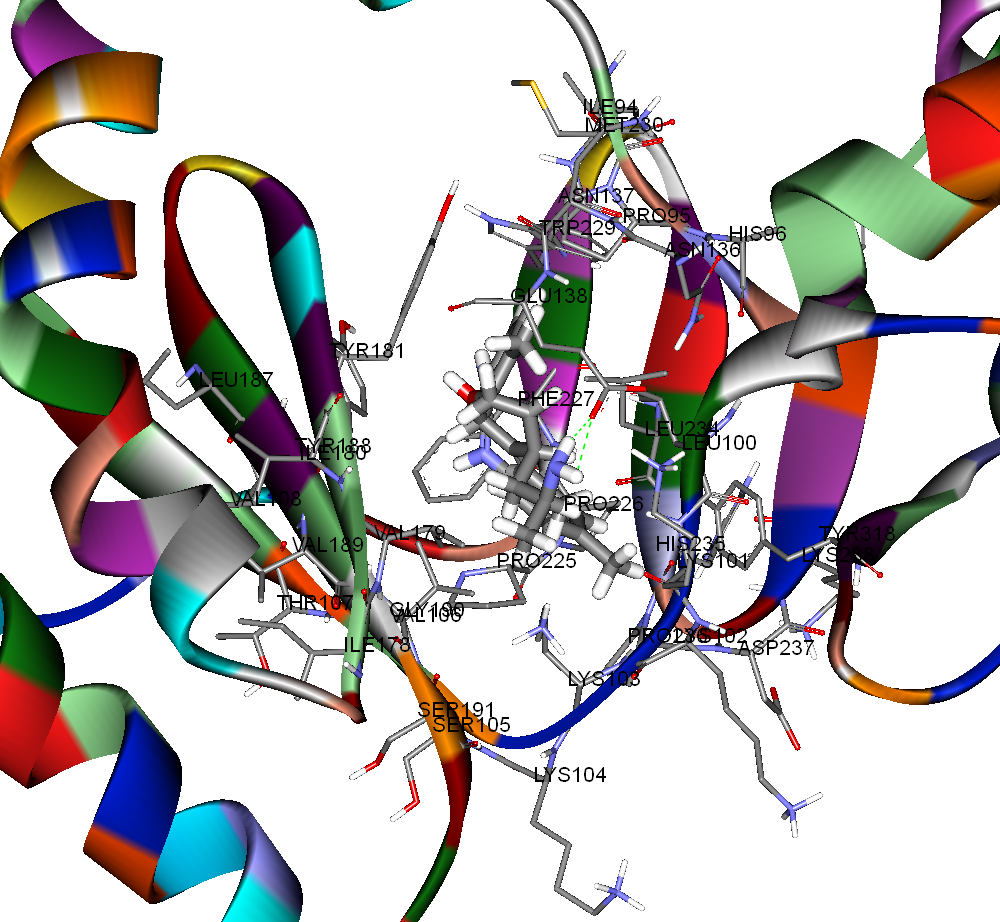
\includegraphics[width=0.3\textwidth]{LigandSynthesis/Figures/Results/2ZD1-ZINC08442219-SmartGrow.png}
  \label{subfig:2ZD1-ZINC08442219-SmartGrow}
}
\subfigure[HIV PR in complex with ZINC20030231.]
{
  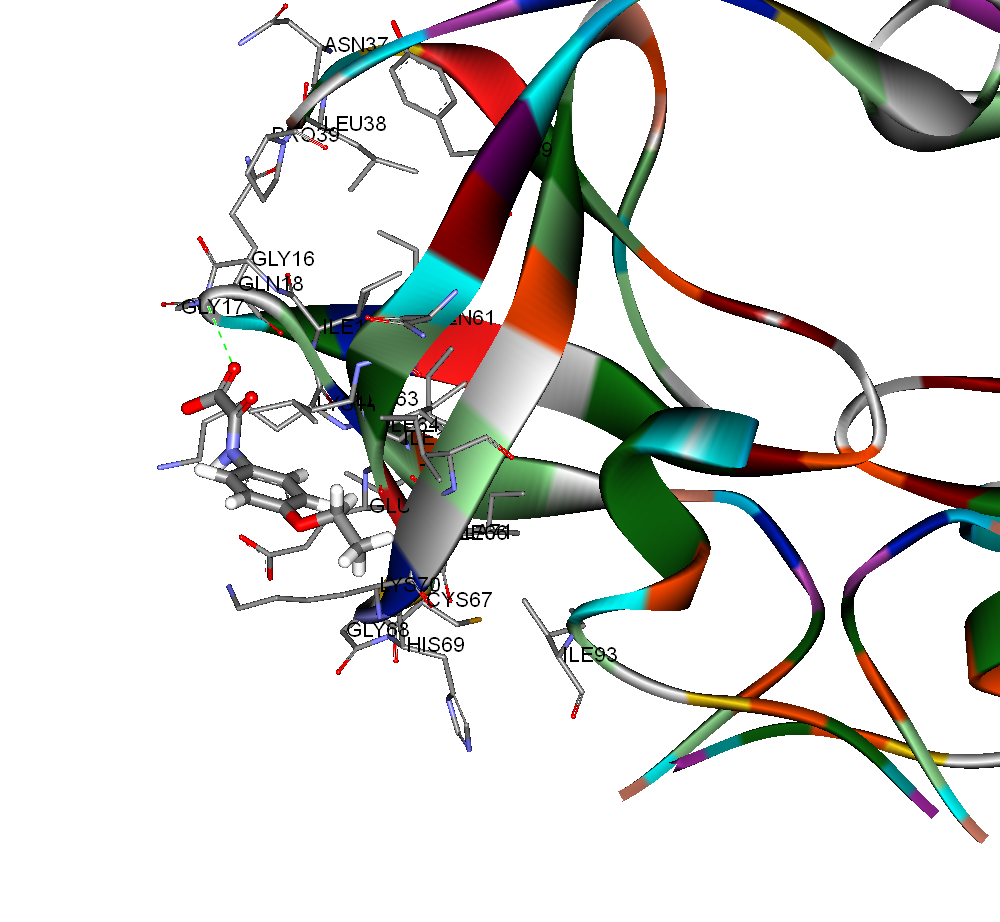
\includegraphics[width=0.3\textwidth]{LigandSynthesis/Figures/Results/3KFN-ZINC20030231.png}
  \label{subfig:3KFN-ZINC20030231}
}
\subfigure[HIV PR in complex with the best generated ligand from ZINC20030231 by AutoGrow.]
{
  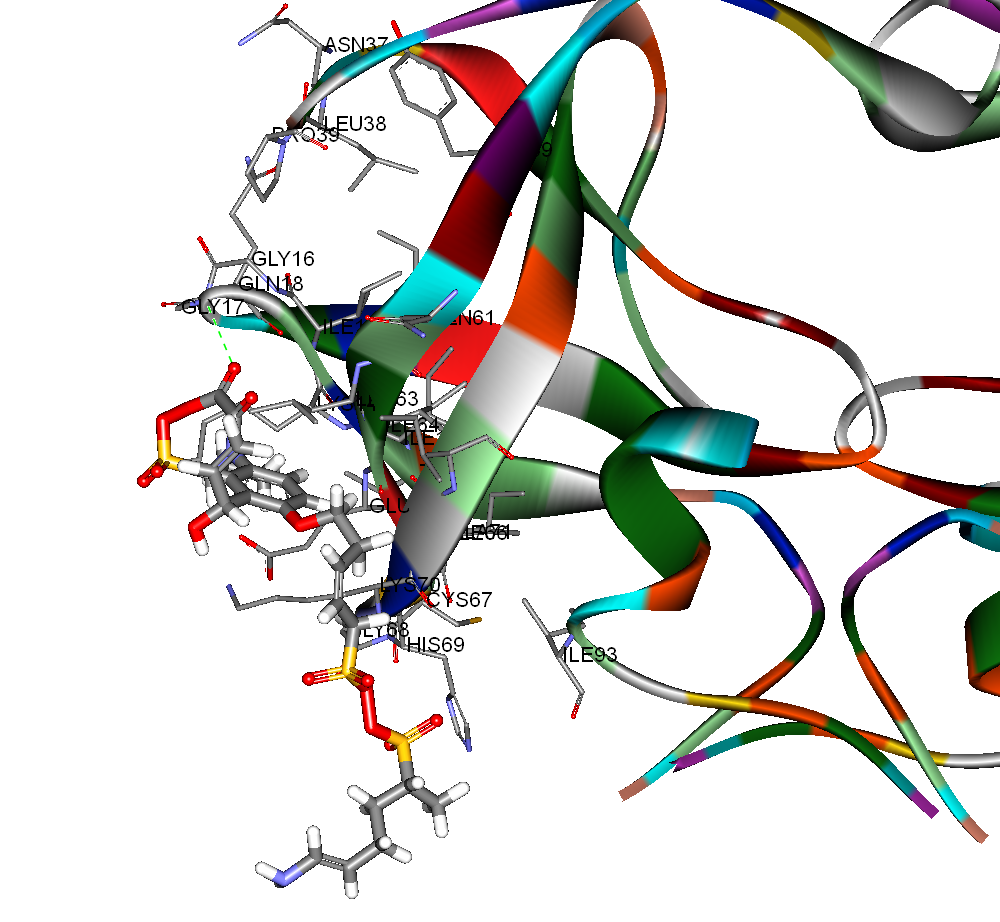
\includegraphics[width=0.3\textwidth]{LigandSynthesis/Figures/Results/3KFN-ZINC20030231-AutoGrow.png}
  \label{subfig:3KFN-ZINC20030231-AutoGrow}
}
\subfigure[HIV PR in complex with the best generated ligand from ZINC20030231 by SmartGrow.]
{
  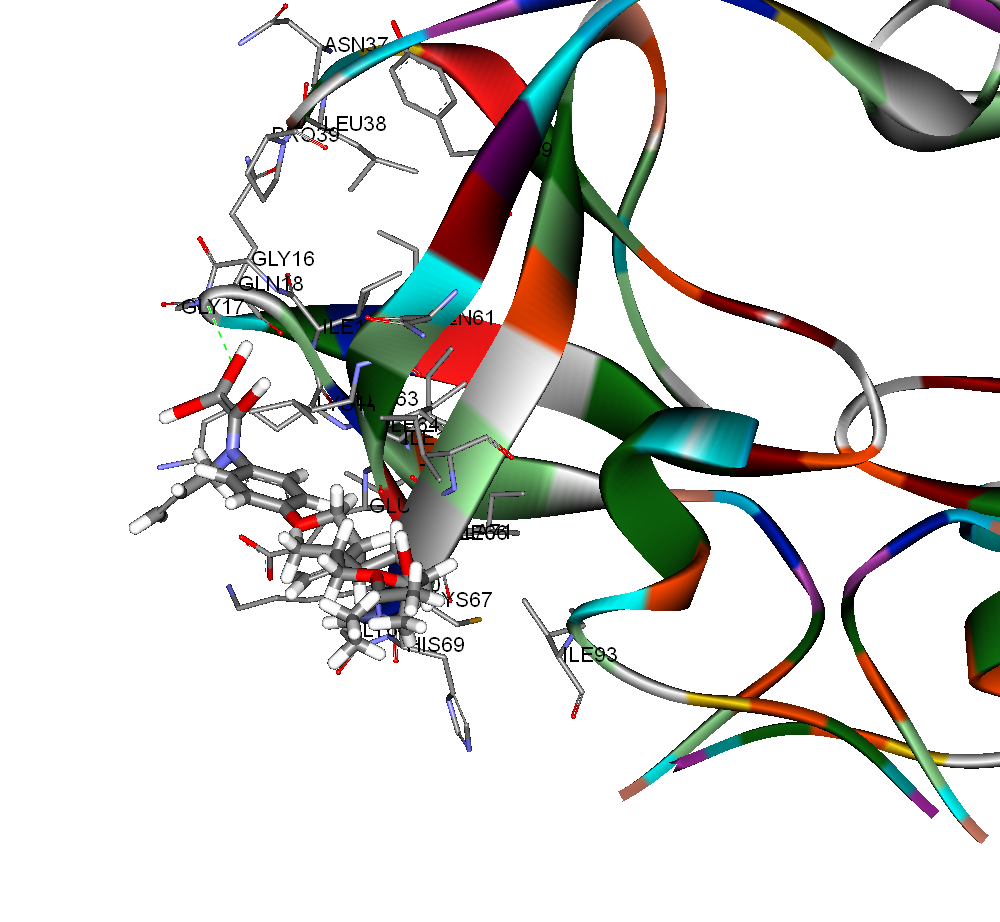
\includegraphics[width=0.3\textwidth]{LigandSynthesis/Figures/Results/3KFN-ZINC20030231-SmartGrow.png}
  \label{subfig:3KFN-ZINC20030231-SmartGrow}
}
\caption{Examples of the best generated ligands by AutoGrow and SmartGrow.}
\label{fig:BestLigands}
\end{figure}

\begin{table}
\centering
\begin{tabular*}
{\textwidth}
{@{\extracolsep{\fill}}lrr}
\toprule
Program & Predicted free energy (kcal/mol) & Molecular Weight (Da)\\
\midrule
\multicolumn{3}{l}{\textbf{ZINC01019824 docked against GSK3$\beta$}}\\
AutoGrow & -11.9 & 572\\
SmartGrow & -11.2 & 505\\
\noalign{\smallskip\smallskip}
\multicolumn{3}{l}{\textbf{ZINC08442219 docked against HIV RT}}\\
AutoGrow & -11.3 & 433\\
SmartGrow & -11.8 & 392\\
\noalign{\smallskip\smallskip}
\multicolumn{3}{l}{\textbf{ZINC20030231 docked against HIV PR}}\\
AutoGrow & -7.3 & 683\\
SmartGrow & -7.5 & 489\\
\bottomrule
\end{tabular*}
\caption{Predicted free energies and molecular weights of the best generated ligands.}
\label{tab:BestLigands}
\end{table}

In the first testcase, the initial ligand ZINC01019824 does not form any hydrogen bond with GSK3$\beta$ (Figure \ref{subfig:1J1B-ZINC01019824}). The best ligand generated by AutoGrow forms 4 hydrogens bonds, interacting with Tyr134, Pro136, Gln185, and Asn186 of GSK3$\beta$ (Figure \ref{subfig:1J1B-ZINC01019824-AutoGrow}). The best ligand generated by SmartGrow forms 9 hydrogens bonds, interacting with Asp133, Tyr134, Pro184, Gln185, and Asn186 of GSK3$\beta$ (Figure \ref{subfig:1J1B-ZINC01019824-SmartGrow}).

In the second testcase, the initial ligand ZINC08442219 does not form any hydrogen bond with HIV RT (Figure \ref{subfig:2ZD1-ZINC08442219}). The best ligand generated by AutoGrow forms 1 hydrogen bond, interacting with Lys101 of chain A of HIV RT (Figure \ref{subfig:2ZD1-ZINC08442219-AutoGrow}). The best ligand generated by SmartGrow forms 2 hydrogen bonds, interacting with Glu138 of chain B of HIV RT (Figure \ref{subfig:2ZD1-ZINC08442219-SmartGrow}).

In the third testcase, the initial ligand ZINC20030231 forms 1 hydrogen bond with HIV PR, interacting with Gly17 of chain A of HIV PR (Figure \ref{subfig:3KFN-ZINC20030231}). The best ligand generated by AutoGrow forms 2 hydrogen bonds, interacting with Lys14 and Gly17 of chain A of HIV PR (Figure \ref{subfig:3KFN-ZINC20030231-AutoGrow}). The best ligand generated by SmartGrow forms 1 hydrogen bond, interacting with Gly17 of chain A of HIV PR (Figure \ref{subfig:3KFN-ZINC20030231-SmartGrow}).

\subsection{Free Energy and Molecule Weight}

The goal of ligand synthesis programs is not to generate one single best ligand, but a population of drug-like ligands for further verifications by wet-lab experiments. Therefore it is more meaningful to dig into the average performance of several best ligands.

Figures \ref{fig:Best5-1J1B}, \ref{fig:Best5-2ZD1}, and \ref{fig:Best5-3KFN} plot the free energies and molecular weights of the best 5 ligands against generation numbers. Generation 0 refers to the initial ligand. Blue curve refers to average free energies of the best 5 ligands generated by AutoGrow. Green curve refers to average free energies of the best 5 ligands generated by SmartGrow. Red curve refers to average molecular weights of the best 5 ligands generated by AutoGrow. Purple curve refers to average molecular weights of the best 5 ligands generated by SmartGrow.

\begin{figure}
\centering
\subfigure[TRS]
{
  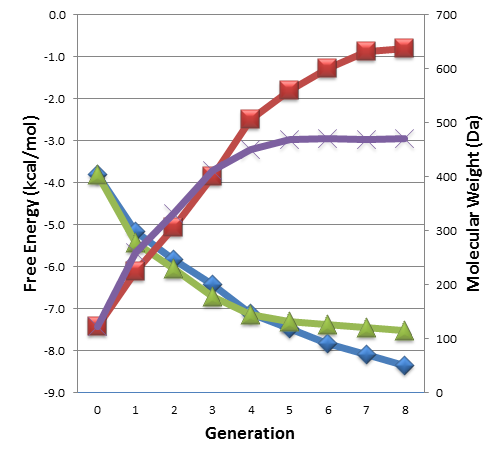
\includegraphics[width=0.45\textwidth]{LigandSynthesis/Figures/Results/Best5-1J1B-TRS.png}
  \label{subfig:Best5-1J1B-TRS}
}
\subfigure[ZINC08442219]
{
  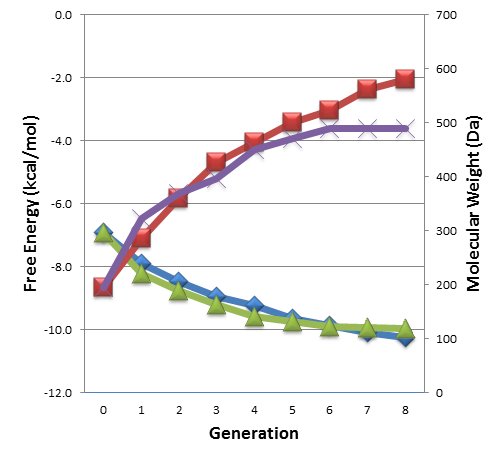
\includegraphics[width=0.45\textwidth]{LigandSynthesis/Figures/Results/Best5-1J1B-ZINC01019824.png}
  \label{subfig:Best5-1J1B-ZINC01019824}
}
\subfigure[ZINC08442219]
{
  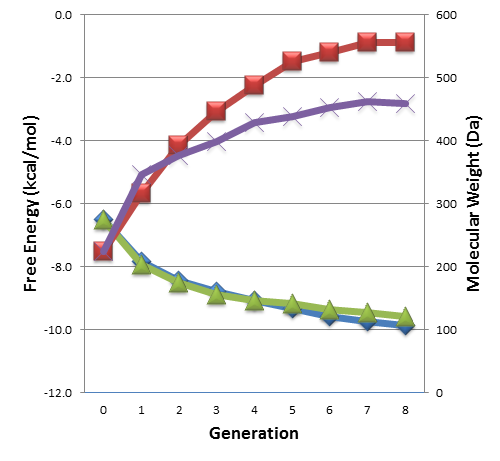
\includegraphics[width=0.45\textwidth]{LigandSynthesis/Figures/Results/Best5-1J1B-ZINC08442219.png}
  \label{subfig:Best5-1J1B-ZINC08442219}
}
\subfigure[ZINC09365179]
{
  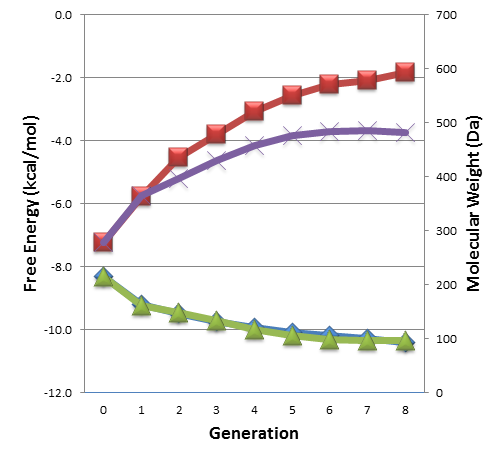
\includegraphics[width=0.45\textwidth]{LigandSynthesis/Figures/Results/Best5-1J1B-ZINC09365179.png}
  \label{subfig:Best5-1J1B-ZINC09365179}
}
\subfigure[ZINC18153302]
{
  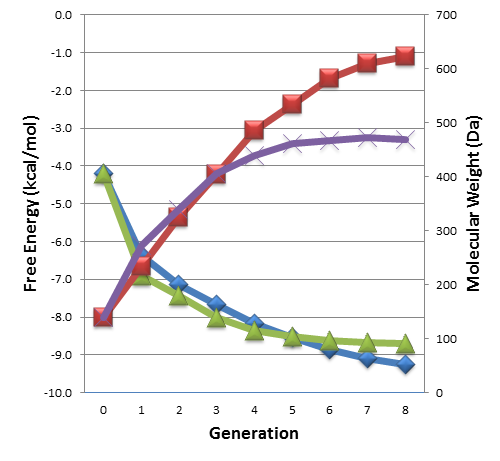
\includegraphics[width=0.45\textwidth]{LigandSynthesis/Figures/Results/Best5-1J1B-ZINC18153302.png}
  \label{subfig:Best5-1J1B-ZINC18153302}
}
\subfigure[ZINC20030231]
{
  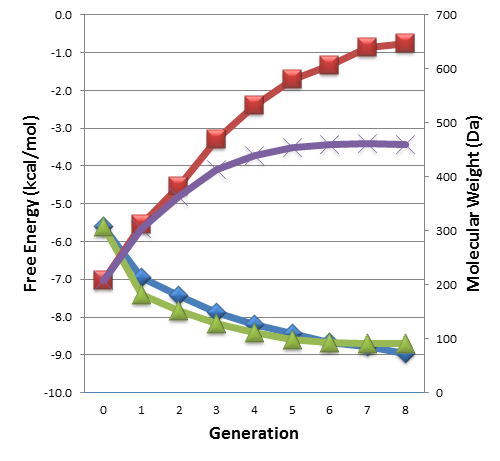
\includegraphics[width=0.45\textwidth]{LigandSynthesis/Figures/Results/Best5-1J1B-ZINC20030231.png}
  \label{subfig:Best5-1J1B-ZINC20030231}
}
\caption{Average free energies and molecular weights of the best 5 ligands generated by AutoGrow and SmartGrow docking against GSK3$\beta$.}
\label{fig:Best5-1J1B}
\end{figure}

\begin{figure}
\centering
\subfigure[T27]
{
  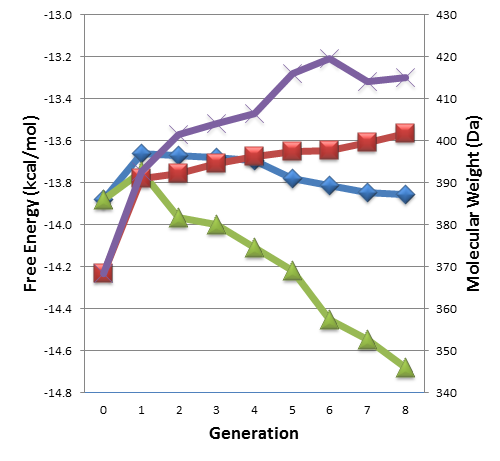
\includegraphics[width=0.45\textwidth]{LigandSynthesis/Figures/Results/Best5-2ZD1-T27.png}
  \label{subfig:Best5-2ZD1-T27}
}
\subfigure[ZINC01019824]
{
  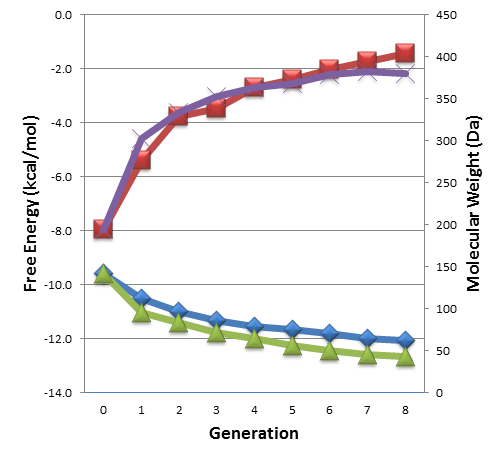
\includegraphics[width=0.45\textwidth]{LigandSynthesis/Figures/Results/Best5-2ZD1-ZINC01019824.png}
  \label{subfig:Best5-2ZD1-ZINC01019824}
}
\subfigure[ZINC08442219]
{
  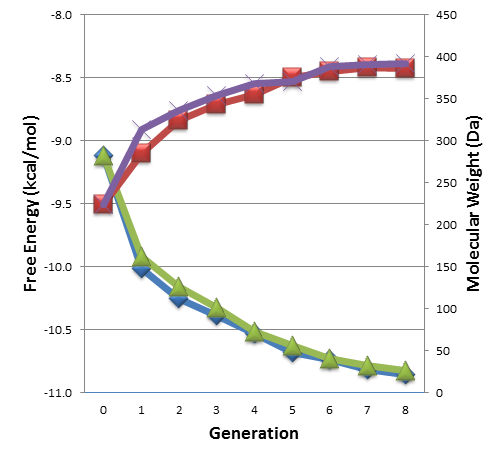
\includegraphics[width=0.45\textwidth]{LigandSynthesis/Figures/Results/Best5-2ZD1-ZINC08442219.png}
  \label{subfig:Best5-2ZD1-ZINC08442219}
}
\subfigure[ZINC09365179]
{
  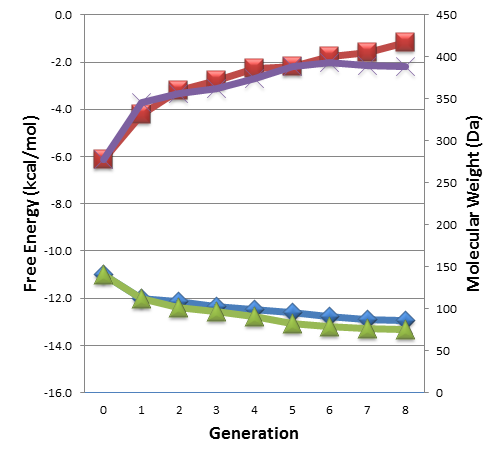
\includegraphics[width=0.45\textwidth]{LigandSynthesis/Figures/Results/Best5-2ZD1-ZINC09365179.png}
  \label{subfig:Best5-2ZD1-ZINC09365179}
}
\subfigure[ZINC18153302]
{
  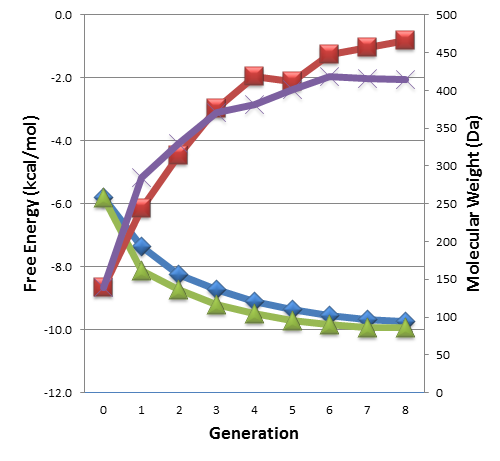
\includegraphics[width=0.45\textwidth]{LigandSynthesis/Figures/Results/Best5-2ZD1-ZINC18153302.png}
  \label{subfig:Best5-2ZD1-ZINC18153302}
}
\subfigure[ZINC20030231]
{
  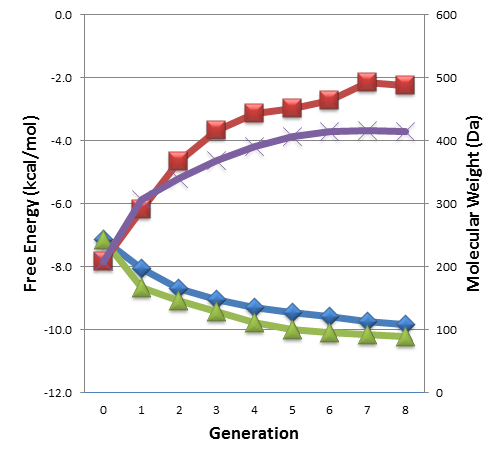
\includegraphics[width=0.45\textwidth]{LigandSynthesis/Figures/Results/Best5-2ZD1-ZINC20030231.png}
  \label{subfig:Best5-2ZD1-ZINC20030231}
}
\caption{Average free energies and molecular weights of the best 5 ligands generated by AutoGrow and SmartGrow docking against HIV RT.}
\label{fig:Best5-2ZD1}
\end{figure}

\begin{figure}
\centering
\subfigure[4DX]
{
  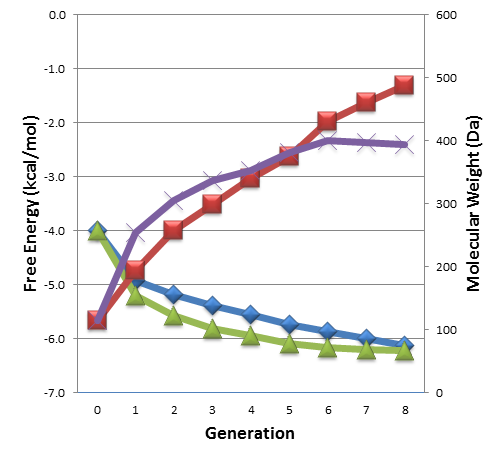
\includegraphics[width=0.45\textwidth]{LigandSynthesis/Figures/Results/Best5-3KFN-4DX.png}
  \label{subfig:Best5-3KFN-4DX}
}
\subfigure[ZINC01019824]
{
  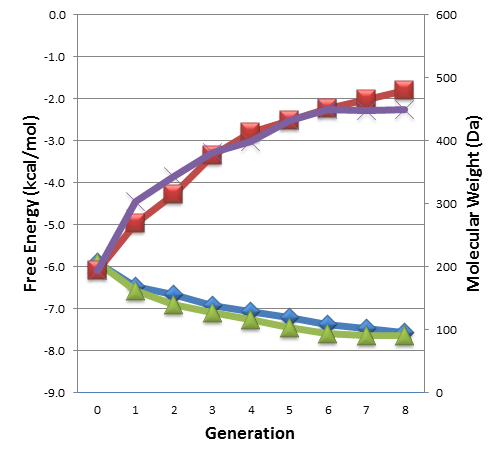
\includegraphics[width=0.45\textwidth]{LigandSynthesis/Figures/Results/Best5-3KFN-ZINC01019824.png}
  \label{subfig:Best5-3KFN-ZINC01019824}
}
\subfigure[ZINC08442219]
{
  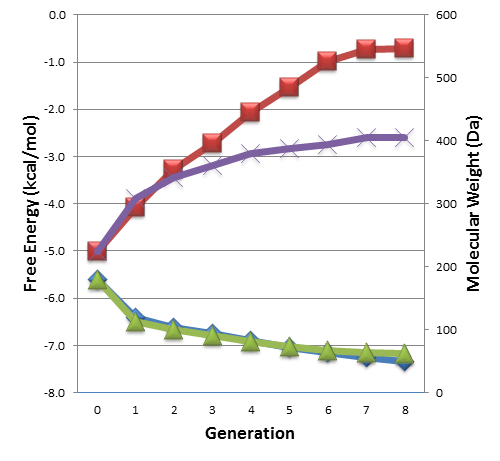
\includegraphics[width=0.45\textwidth]{LigandSynthesis/Figures/Results/Best5-3KFN-ZINC08442219.png}
  \label{subfig:Best5-3KFN-ZINC08442219}
}
\subfigure[ZINC09365179]
{
  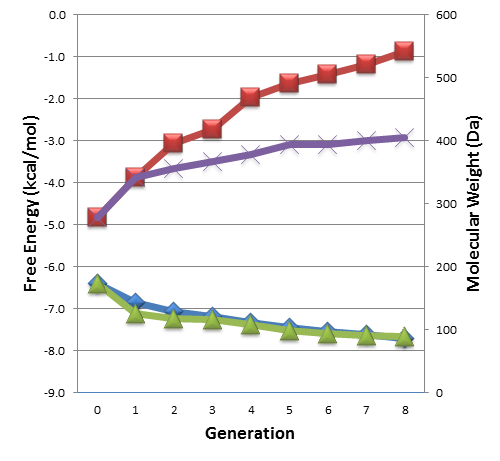
\includegraphics[width=0.45\textwidth]{LigandSynthesis/Figures/Results/Best5-3KFN-ZINC09365179.png}
  \label{subfig:Best5-3KFN-ZINC09365179}
}
\subfigure[ZINC18153302]
{
  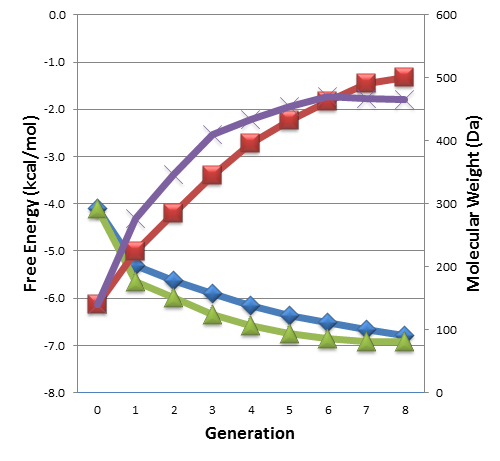
\includegraphics[width=0.45\textwidth]{LigandSynthesis/Figures/Results/Best5-3KFN-ZINC18153302.png}
  \label{subfig:Best5-3KFN-ZINC18153302}
}
\subfigure[ZINC20030231]
{
  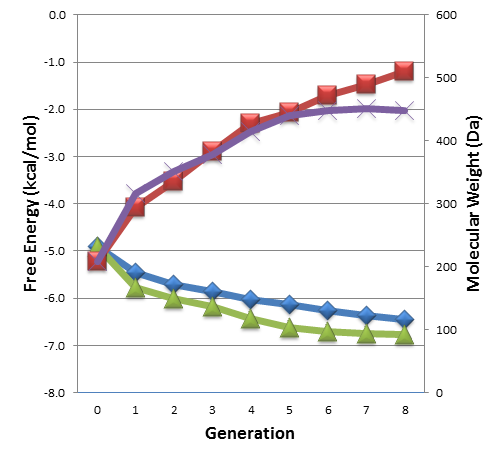
\includegraphics[width=0.45\textwidth]{LigandSynthesis/Figures/Results/Best5-3KFN-ZINC20030231.png}
  \label{subfig:Best5-3KFN-ZINC20030231}
}
\caption{Average free energies and molecular weights of the best 5 ligands generated by AutoGrow and SmartGrow docking against HIV PR.}
\label{fig:Best5-3KFN}
\end{figure}

\subsection{Execution Time}

We also measured the execution times of AutoGrow and SmartGrow for running all the 18 testcases for 9 times. Figures \ref{fig:SynthesisExecutionTime} and \ref{fig:SynthesisSpeedup} show their average execution times and the speedups of SmartGrow over AutoGrow. A positive speedup value indicates SmartGrow ran faster than AutoGrow in that testcase, while a negative speedup value indicates SmartGrow ran slower.

\begin{figure}[t]
\centering
\subfigure[GSK3$\beta$]
{
  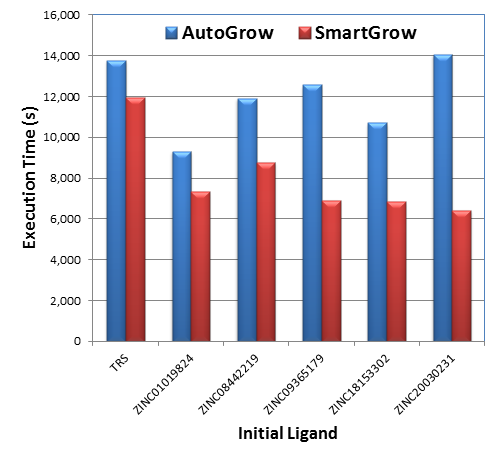
\includegraphics[width=0.3\textwidth]{LigandSynthesis/Figures/Results/ExecutionTime-1J1B.png}
  \label{subfig:ExecutionTime-1J1B}
}
\subfigure[HIV RT]
{
  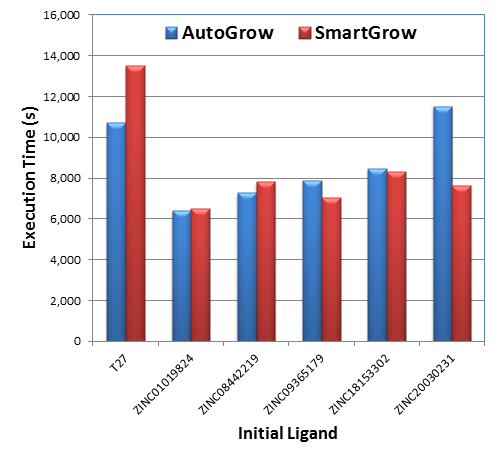
\includegraphics[width=0.3\textwidth]{LigandSynthesis/Figures/Results/ExecutionTime-2ZD1.png}
  \label{subfig:ExecutionTime-2ZD1}
}
\subfigure[HIV PR]
{
  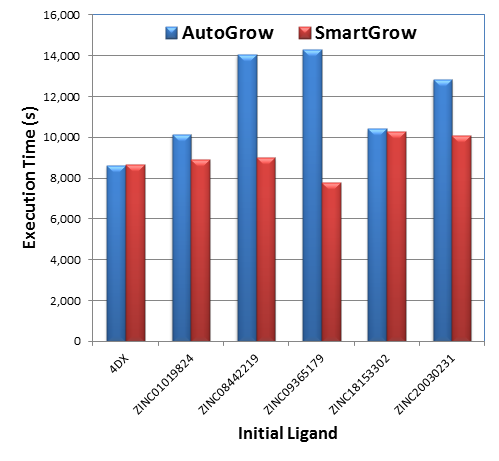
\includegraphics[width=0.3\textwidth]{LigandSynthesis/Figures/Results/ExecutionTime-3KFN.png}
  \label{subfig:ExecutionTime-3KFN}
}
\caption{Average execution times of AutoGrow and SmartGrow.}
\label{fig:SynthesisExecutionTime}
\end{figure}

\begin{figure}
\centering
\subfigure[GSK3$\beta$]
{
  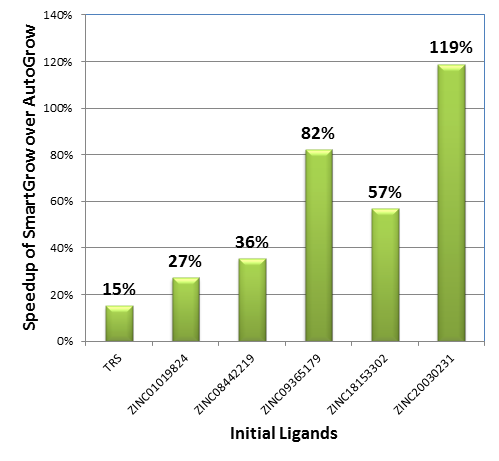
\includegraphics[width=0.3\textwidth]{LigandSynthesis/Figures/Results/Speedup-1J1B.png}
  \label{subfig:Speedup-1J1B}
}
\subfigure[HIV RT]
{
  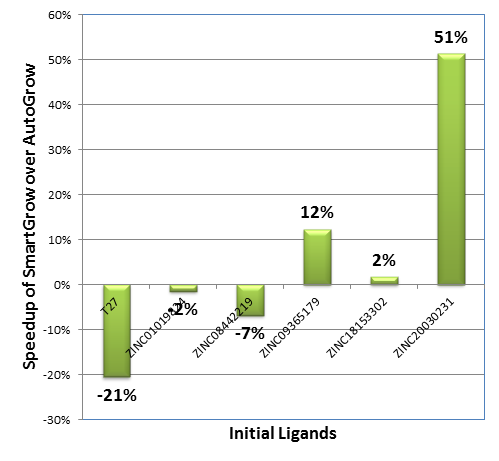
\includegraphics[width=0.3\textwidth]{LigandSynthesis/Figures/Results/Speedup-2ZD1.png}
  \label{subfig:Speedup-2ZD1}
}
\subfigure[HIV PR]
{
  \includegraphics[width=0.3\textwidth]{LigandSynthesis/Figures/Results/Speedup-3KFN.png}
  \label{subfig:Speedup-3KFN}
}
\caption{Average speedups of SmartGrow over AutoGrow.}
\label{fig:SynthesisSpeedup}
\end{figure}

\subsection{Support for Phosphorus}

SmartGrow has built-in support for the chemical element of phosphorus. To test such capability, we picked an additional phosphorus-containing ligand with heterogeneous molecule ID of TFO from PDB, and generated ligands from TFO docking against HIV reverse transcriptase. Figure \ref{fig:TFO} demonstrates the capability of handling phosphorus by SmartGrow.

\begin{figure}
\centering
\subfigure[The best ligand generated by SmartGrow.]
{
  \includegraphics[width=0.65\textwidth]{LigandSynthesis/Figures/Results/2ZD1-TFO-SmartGrow.png}
  \label{subfig:2ZD1-TFO-SmartGrow}
}
\subfigure[Average free energies and molecular weights of the best 5 ligands generated from TFO by SmartGrow docking against HIV RT.]
{
  \includegraphics[width=0.65\textwidth]{LigandSynthesis/Figures/Results/Best5-2ZD1-TFO.png}
  \label{subfig:Best5-2ZD1-TFO}
}
\caption{SmartGrow results of docking TFO against HIV RT.}
\label{fig:TFO}
\end{figure}

\section{Discussion}

Through visualizing the generated ligands in complex of their respective protein, we found that they are chemically valid, verifying the correctness of of both programs.

Regarding the number of hydrogen bonds that the best generated ligand can form with the protein (Figure \ref {fig:BestLigands}), both programs display similar performance. Nevertheless, the best ligands generated by SmartGrow have significantly lower molecular weights, hence they have greater potential to optimize into drugs.

Regarding the average free energies and molecular weights of the best 5 ligands generated by both programs (Figures \ref{fig:Best5-1J1B}, \ref{fig:Best5-2ZD1}, and \ref{fig:Best5-3KFN}), SmartGrow displays comparable free energy curves for most of the cases, while its molecular weight curves are remarkably lower than AutoGrow, and never exceed 500 Da thanks to the guidance of Lipinski's \textit{Rule of Five}.

Regarding the execution time (Figure \ref{fig:SynthesisExecutionTime}), SmartGrow outperforms AutoGrow for 14 out of 18 testcases. For the testcase with GSK3$\beta$ as the protein and ZINC20030231 as the initial ligand, SmartGrow runs as much as 119\% faster than AutoGrow (Figure \ref{subfig:Best5-1J1B-ZINC20030231}). For the testcase with HIV RT as the protein and T27 as the initial ligand, although SmartGrow requires 27\% more time, the generated ligands have lower free energies (Figure \ref{subfig:Best5-2ZD1-T27}). Averaging all the 18 testcases, SmartGrow executes 30\% faster than AutoGrow.

\section{Availability}

SmartGrow is free and open source under no license, available at http://www.cse.cuhk.edu.hk/\textasciitilde hjli/smartgrow.tar.gz

\section{Conclusion}

We have developed SmartGrow, an efficient tool for computational synthesis of potent ligands. SmartGrow inherits the mutation and crossover operators from AutoGrow, and invents two new genetic operators, namely split and merging, significantly enriching ligand diversity. The split operator ensures that ligands will not grow excessively large. The merging operator is basically a reversed operator of split and aims to accelerate ligand growing. SmartGrow implements Lipinski's \textit{Rule of Five} \citep{168-2004} to ensure drug likeness. The program design is so flexible that it reserves room for adaptation to new chemical constraints. Its robust parser correctly processes two-letter chemical elements, and meanwhile adds additional support for phosphorus. The results show that SmartGrow outperforms AutoGrow in terms of free energy, molecular weight, and execution time.

In conclusion, SmartGrow demonstrates superior performance and is proved to be an efficient tool for computational synthesis of potent ligands for drug discovery. Improving ligand specificity \citep{473-2010} is scheduled as future work.

\section{Personal Contribution}

The development of SmartGrow is the result of teamwork with my colleague Benjamin Ching-Man Tse. I started working on developing SmartGrow in April 2010. I proposed the ideas of scoring without docking as well as the split operator, implemented part of the program for the interface with Vina, collected the entire testcases including 3 receptors and 18 initial ligands, performed initial docking, set up the running environments on 6 Linux machines, performed massive ligand synthesis, ran both SmartGrow and AutoGrow for 9 times for each testcase, calculated the program execution times, summarized raw data into spreadsheets, drew tables, plotted charts, analyzed results in multiple dimensions, and made concrete conclusions.

\chapterend
